\section{引言}
%%%%%%%%%%%%% Background %%%%%%%%%%%%%
与其他智能设备(智能手机和物联网设备)不同,无人机是一种无人驾驶飞行器,可提供各种自动化功能以支持自主操作。
由于无人机在关键任务中的使用日益增多~\cite{hassija2021fast, sharma2020communication},客户对无人机飞行的可靠性和稳定性提出了更高的要求。
为了以自动化方式控制无人机的运动并保持安全飞行,需要使用控制程序来执行从不同传感器收集数据并生成控制输出以稳定飞行状态的任务。
为了使控制程序更具适应性,无人机操作员可以配置大量的\emph{控制参数},这些参数是限制无人机某些行为的数值(例如,允许的最大角度变化速度)。
由于这些控制参数直接影响控制程序,因此对无人机的飞行安全至关重要。

%%%%%%%%%%%%% The importance of realtime control parameter configuration %%%%%%%%%%%%%
尽管控制参数非常重要,但目前大多数无人机都没有提供简单易用且功能强大的参数配置机制,因此往往需要非专业的人类操作员来完成这项配置任务。
更糟糕的是,由于\emph{范围规范错误(Range Specification Bugs}~\cite{rvfuzzer,han2022control},一种由于控制程序错误设置控制参数范围规范而导致的错误),一些控制程序甚至接受故意配置错误的控制参数,这将导致不稳定的物理状态,最终导致无人机坠毁或飞行任务中断。

%%%%%%%%%%%%% Existing works and their weaknesses %%%%%%%%%%%%%
为了保证控制参数的正确配置,许多防御系统会静态检查已配置的控制参数,防止参数设置不当。
遗憾的是,它们无法有效防止外部物理攻击~\cite{choi2018detecting, quinonez2020savior, dash2019out, tippenhauer2011requirements, son2015rocking, fadilahBLC20, trippel2017walnut}或飞行过程中针对无人机的恶意注入~\cite{rvfuzzer, han2022control, zhou2022doublestar}等主动攻击。
这些攻击通过破坏无人机物理状态的稳定来干扰飞行,而默认的控制参数无法适应这种干扰,从而导致坠毁或严重偏离计划飞行路径等严重后果,最终导致无人机无法到达目的地,造成任务失败。
由于这些威胁只能在飞行过程中识别,因此现有的在代码层面修复漏洞的静态修复方法不适用于飞行控制程序~\cite{kim2022pgpatch, mayday, qi2014strength, kim2022reverse}。
虽然有人提出了一些动态方法来修复漏洞,但其目标是代码逻辑漏洞而非物理不稳定性。
部分方法~\cite{choi2020software, dash2021pid}采用冗余控制算法,在检测到异常情况时接管无人机。
但是,这些方法需要修改代码,而且只适用于特定的无人机,往往会带来额外的开销。
此外,一些解决方案~\cite{rvfuzzer, han2022control}侧重于通过限制无人机的操作空间来提高安全性。
但这些预设限制并不适合所有飞行情况,而且缺乏灵活性。

避免直接修改控制程序中的原始飞行控制算法,更好的解决方案是为无人机引入自动自适应控制参数矫正机制:
在飞行过程中,一旦控制参数被恶意篡改,或者飞行需要一套新的控制参数来处理物理干扰,矫正机制就能立即修复现有的不合适配置,以保持无人机的稳定。
然而,开发实时控制参数矫正方法非常具有挑战性。
一个主要障碍是如何有效地矫正控制参数。
一方面,目前的无人机计算机单元硬件(例如,\tool{Pixhawk}~\cite{meier2011pixhawk}和\tool{TauLabs}~\cite{ebeid2018survey})都基于\tool{STM32}或\tool{ARM}等轻量级板载芯片,计算能力有限。
由于无人机需要分配大部分资源来确保控制算法的运行,因此无法运行需要大量计算资源的复杂算法或冗余组件。
另一方面,尽管矫正需要完成一系列复杂任务,即识别不稳定趋势并生成矫正配置以驱动无人机趋于稳定,但完成矫正的时间窗口非常小(通常只有几秒钟)。


%%%%%%%%%%%%% Our solution %%%%%%%%%%%%%
本章节提出了一种基于强化学习的可靠子啊先修复方案,并实现了原型系统\nyctea,该系统通过增加监测和实时矫正控制参数来缓解攻击造成的不稳定性。
为了实现目标,\nyctea 配备了两个基本功能。
第一个功能是通过实时监控无人机的状态偏差来确定无人机是否处于不稳定的物理状态。
它捕捉一段与飞行相关的数据,计算整体状态偏差,从而确定不稳定趋势。
第二项功能是使用强化学习智能体将现有的控制参数矫正为最合适的值。
其中使用的矫正经验是智能体通过反复修正飞行中遇到的造成不稳定的配置来积累的。



\section{实际影响与挑战}
尽管无人机制造商开发了自动驾驶飞行器的飞行控制程序,但对于不同类型的无人机,必须对一组(通常是数百个)控制参数进行配置,以建议允许的值。
然而,正如上一大章节所介绍的,当前的控制参数配置过程缺乏灵活性~\cite{avola2021automatic},因为它们往往无法支持空中自动调整。
本章节的目标是使用更加灵活的方案改进控制参数配置的使用并实现自动飞行调整。
本章希望为当前的无人机引入一种实时控制参数矫正机制,帮助它们在飞行过程中根据遇到的事件(如人为乱流或传感器欺骗攻击)持续调整参数值,或抵御恶意配置注入攻击~\cite{rvfuzzer, han2022control}。
在结合\icsearcher 的情况先,在起飞前和起飞后的双场景下共同保证飞行安全。


\subsection{预先实验}
本预实验将解释了无人机飞行状态在手动不正确配置的影响下,如何从稳定状态变为不可控状态的三个连续阶段。

\subsubsection{模拟不正确}
本预实验对装有开源飞行控制程序(\tool{Ardupilot}~\cite{ardupilot})的无人机上传了四种不正确配置,以诱发不稳定的物理状态(即偏航和盘旋),导致最终失控。
具体来说,实验首先随机设定一个飞行任务,然后在飞行过程中发上传已经经过确认的不正确配置,这四个配置会通过造成无人机无法正确完成飞行任务。
图~\ref{fig:unstable_example} 展示了所造成的物理轨迹变化,其中绿点和橙点分别代表起飞点和航点,黑虚线为任务规划中的飞行路径,红线为实现轨迹。

\begin{figure}[htb]
\centering{
\subfloat[轨迹偏航]{\label{subfig:exp_deviation}
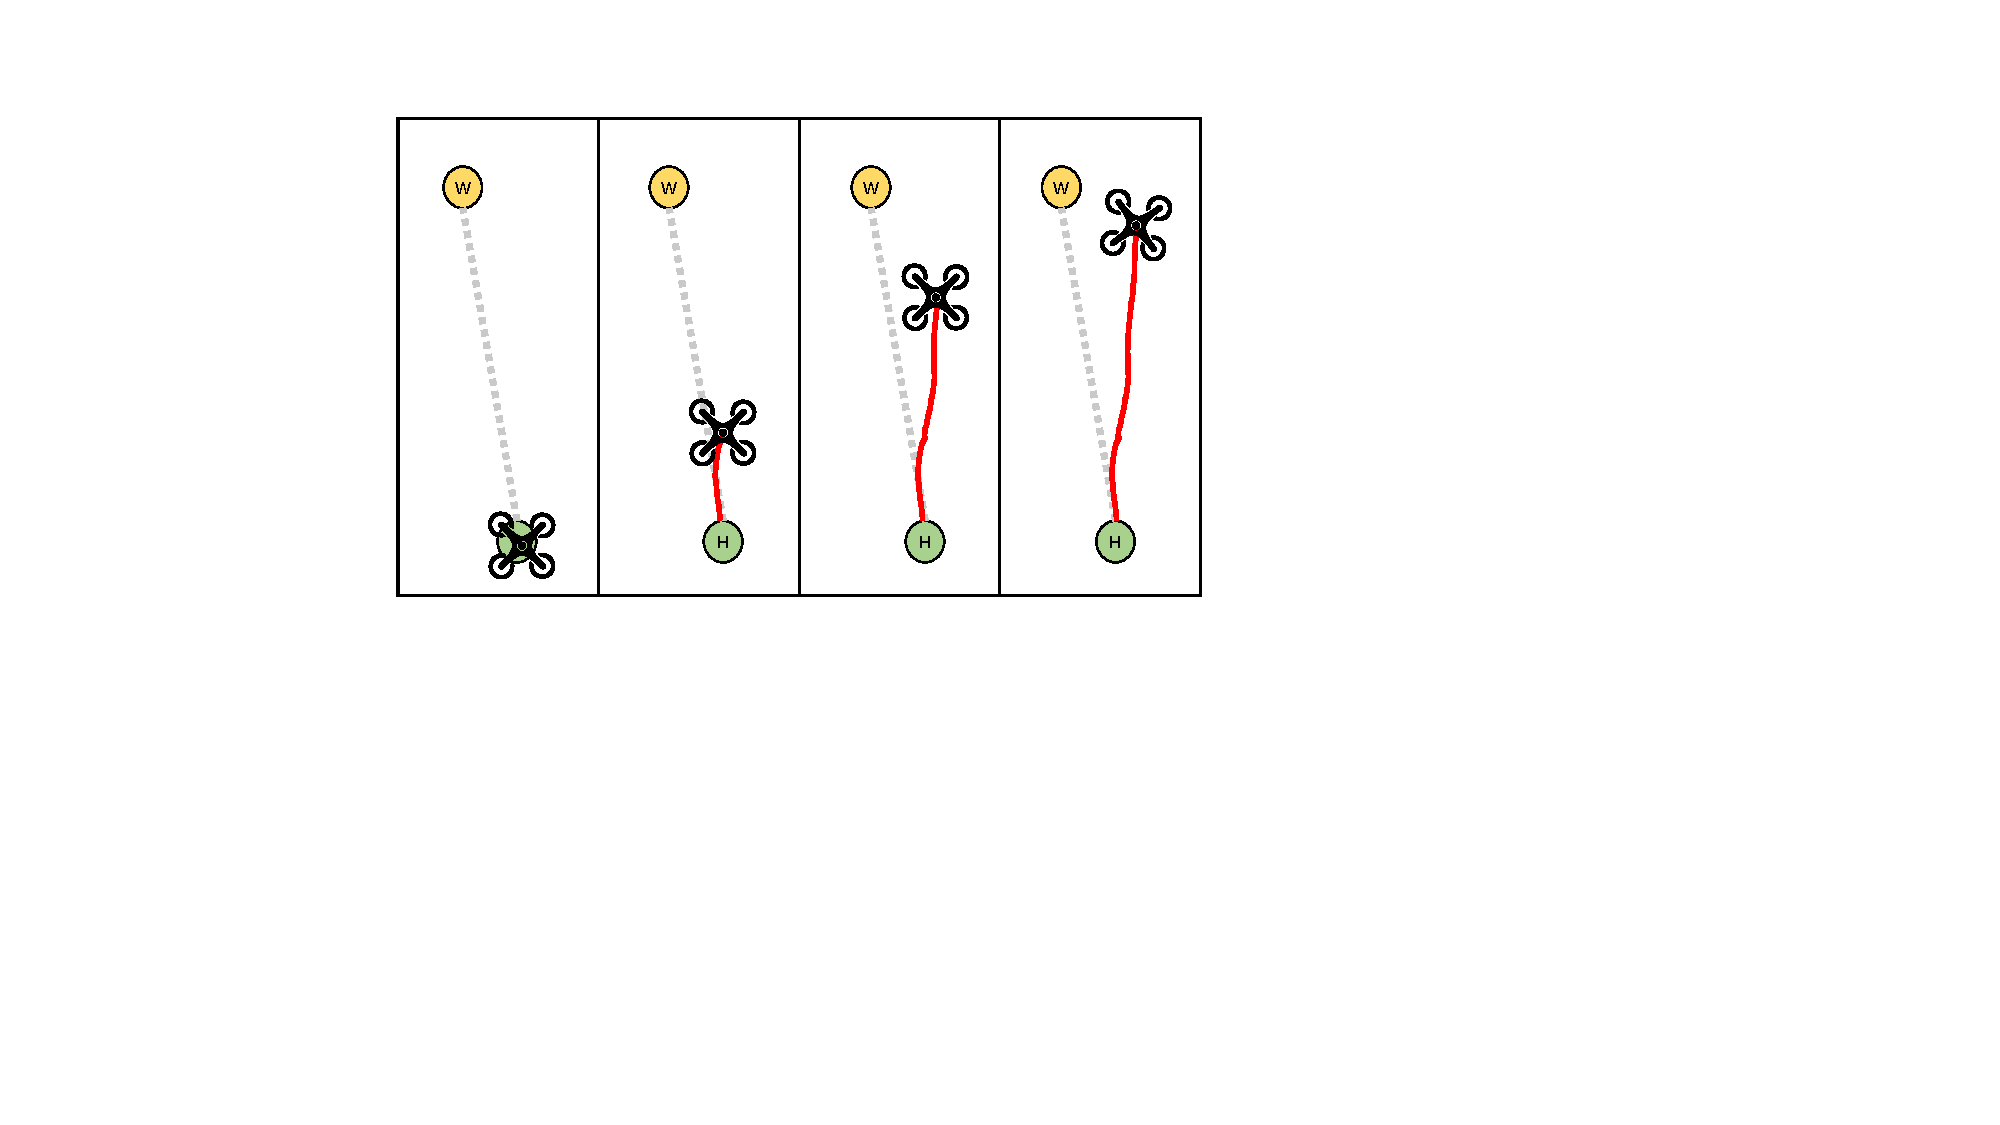
\includegraphics[width=0.48\linewidth]{fig/fix/unstable/deviation.pdf}
}
\subfloat[飞行冻结]{\label{subfig:exp_frozen}
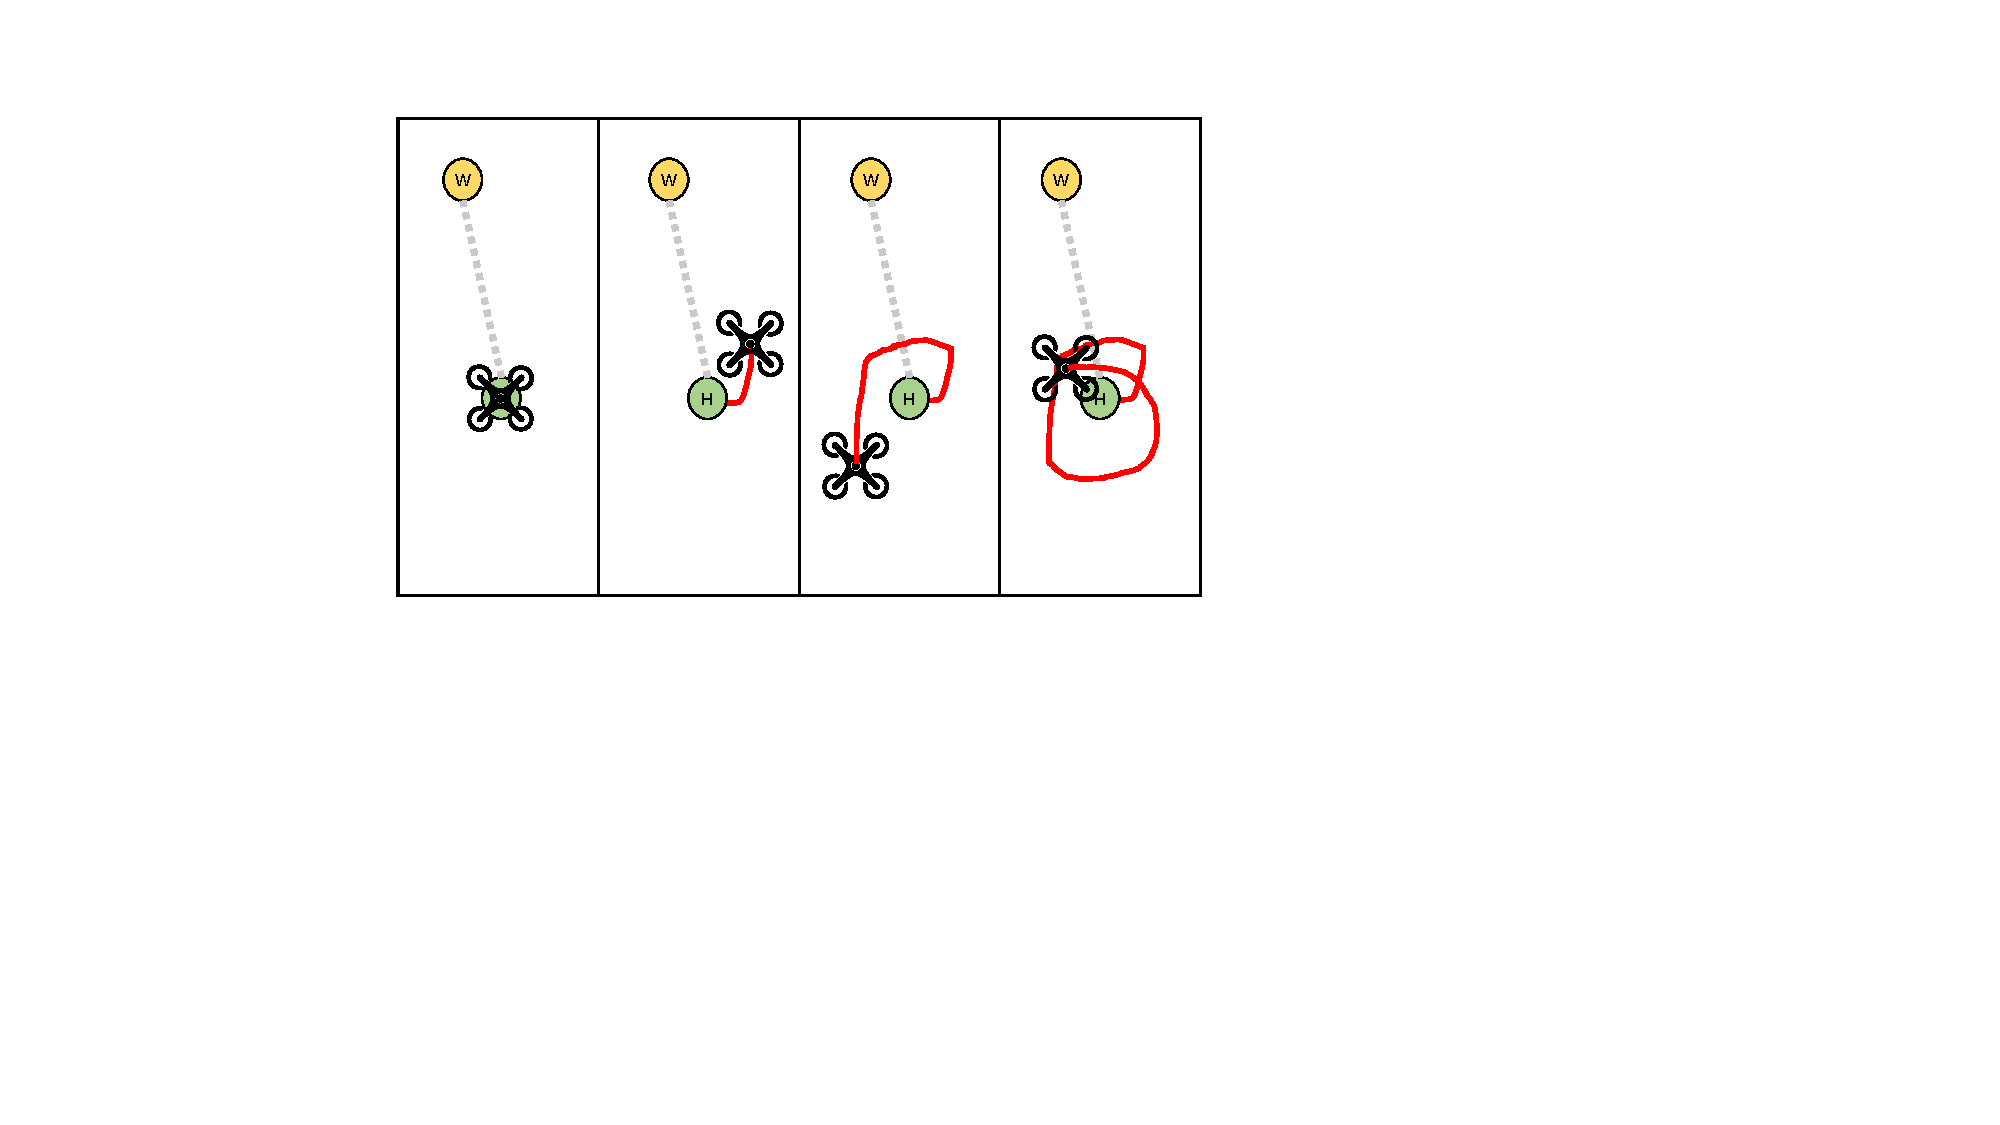
\includegraphics[width=0.48\linewidth]{fig/fix/unstable/frozen.pdf}}
}
\\
\subfloat[飞行坠毁]{\label{subfig:exp_crash}
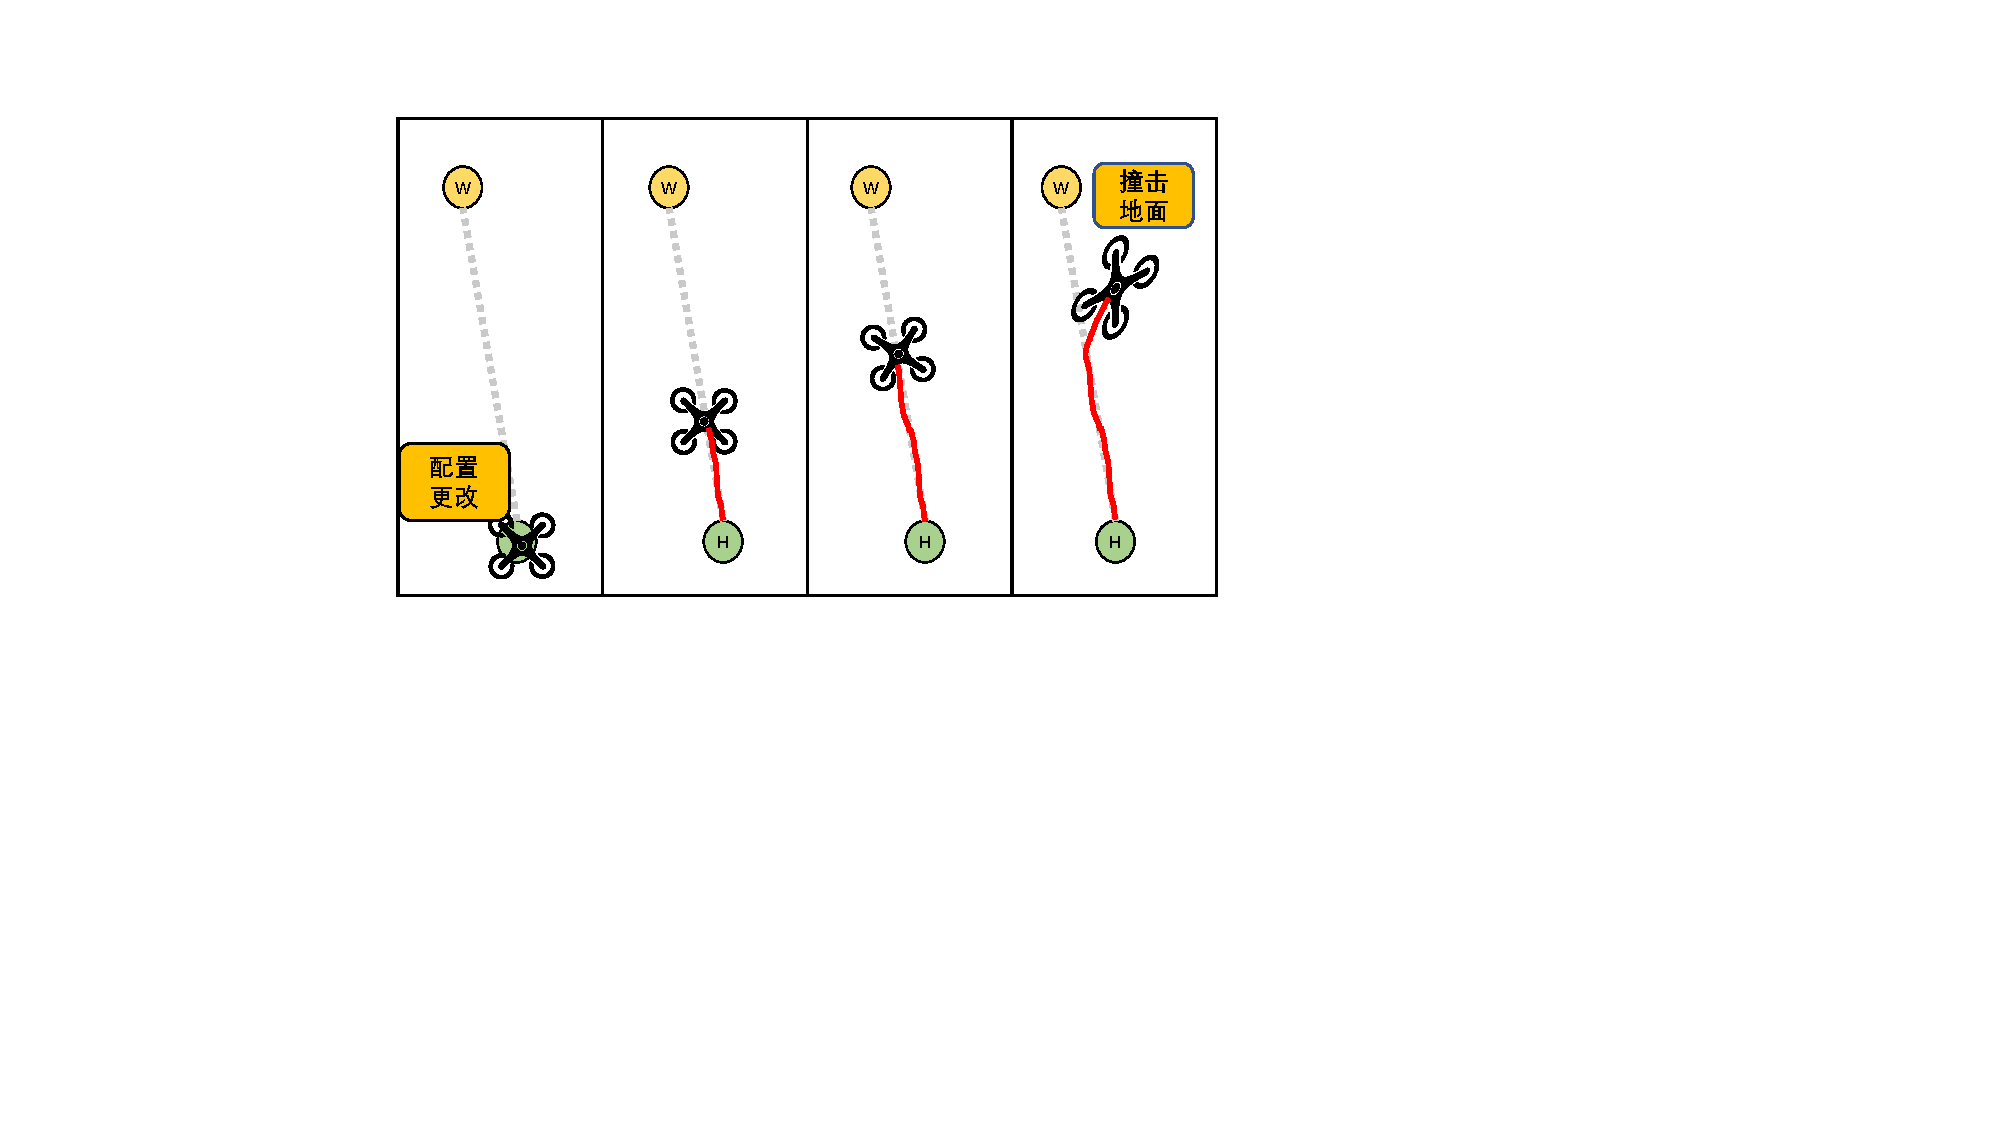
\includegraphics[width=0.48\linewidth]{fig/fix/unstable/crash.pdf}
}
\subfloat[动力损失]{\label{subfig:exp_thrust_loss}
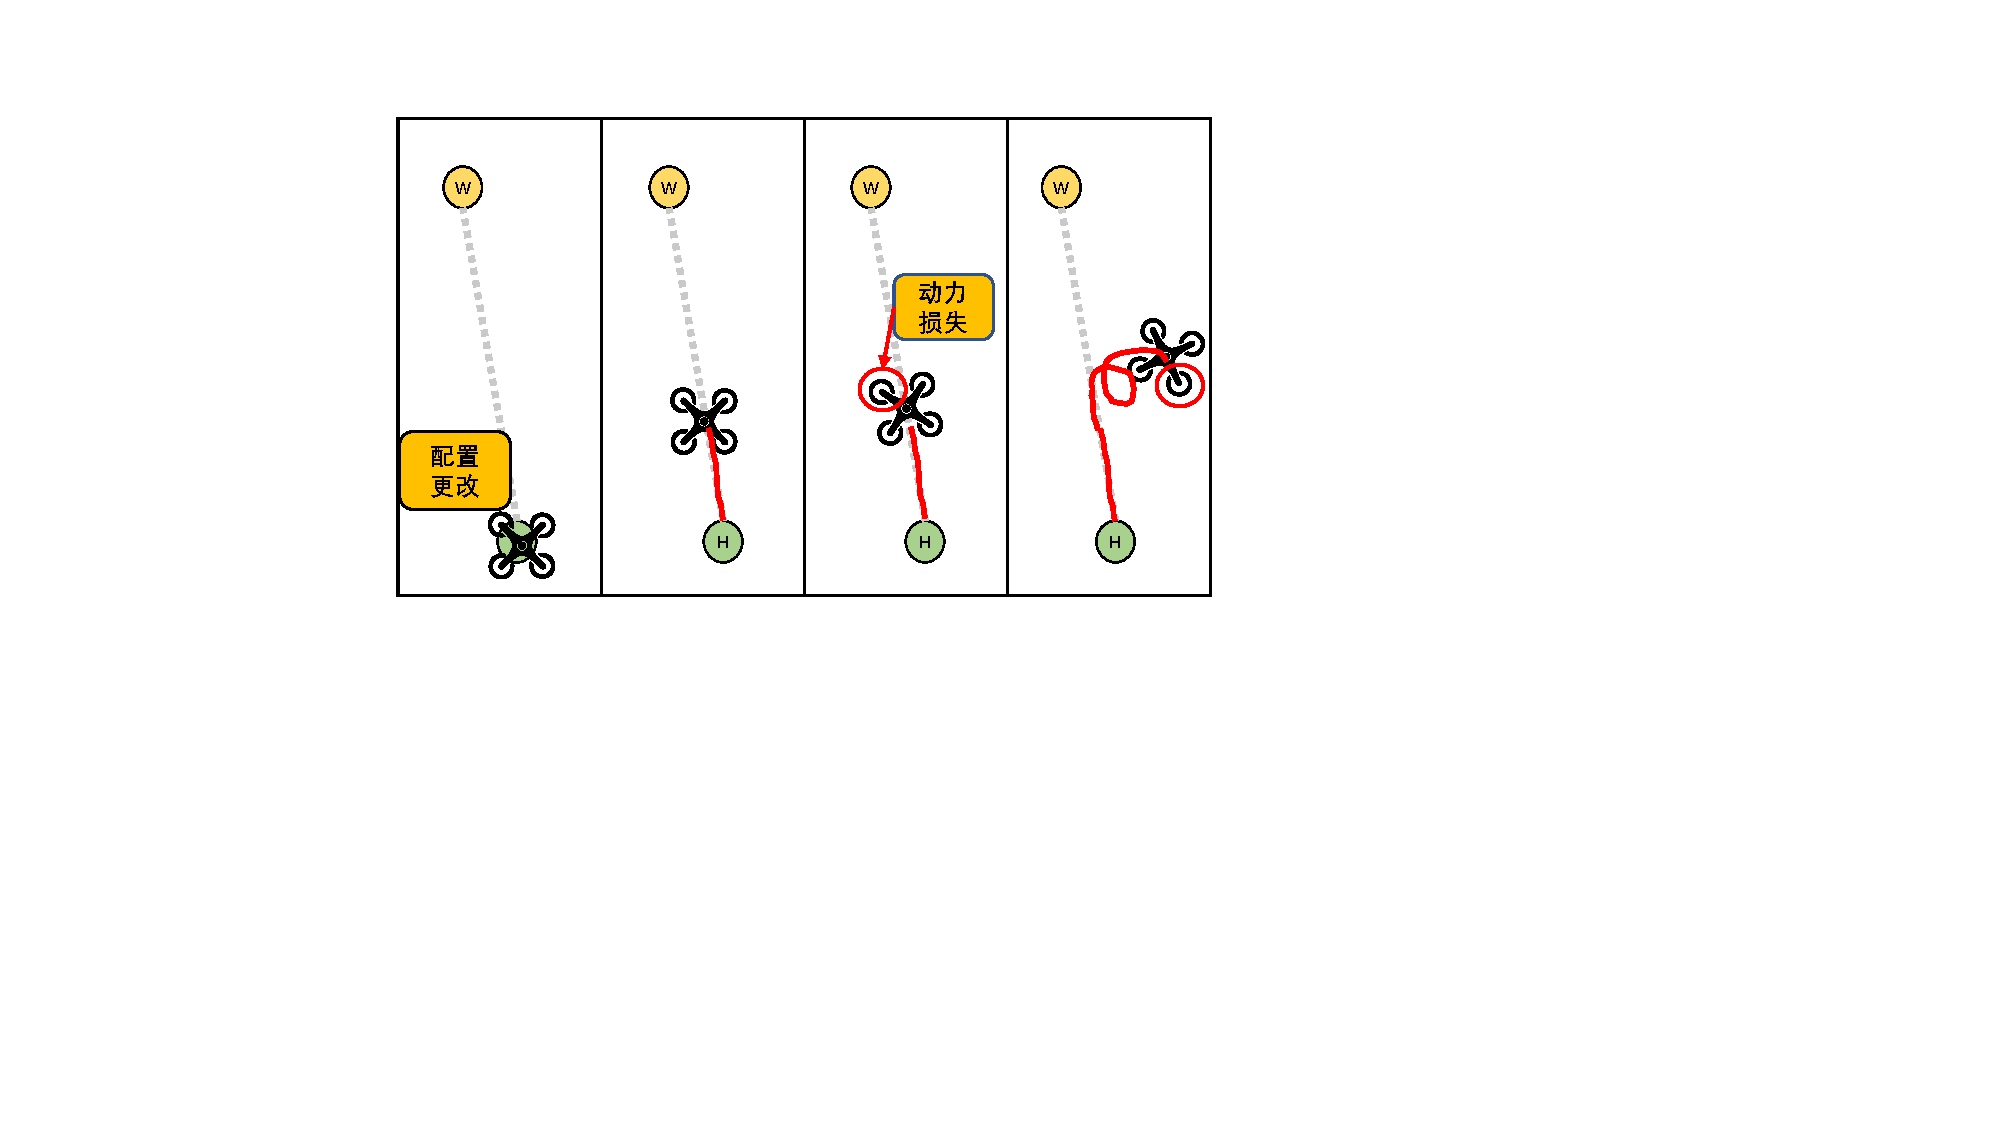
\includegraphics[width=0.48\linewidth]{fig/fix/unstable/thrust loss.pdf}}

\caption{四个不稳定物理状态示例的轨迹。}
\label{fig:unstable_example}
\end{figure}


\subsubsection{攻击下的状态变化}
为了更好地说明\dquote{如何评估和确定控制参数矫正的最佳时机},本预实验手动检查了攻击前后的状态变化,并记录了变化阶段。
以轨迹造成偏航的的配置攻击为例,图~\ref{fig:frozen_state} 分别展示了Roll、Pitch和Yaw角度变化的波动。

\begin{figure}[htb]
\centering{
\label{subfig:raw}
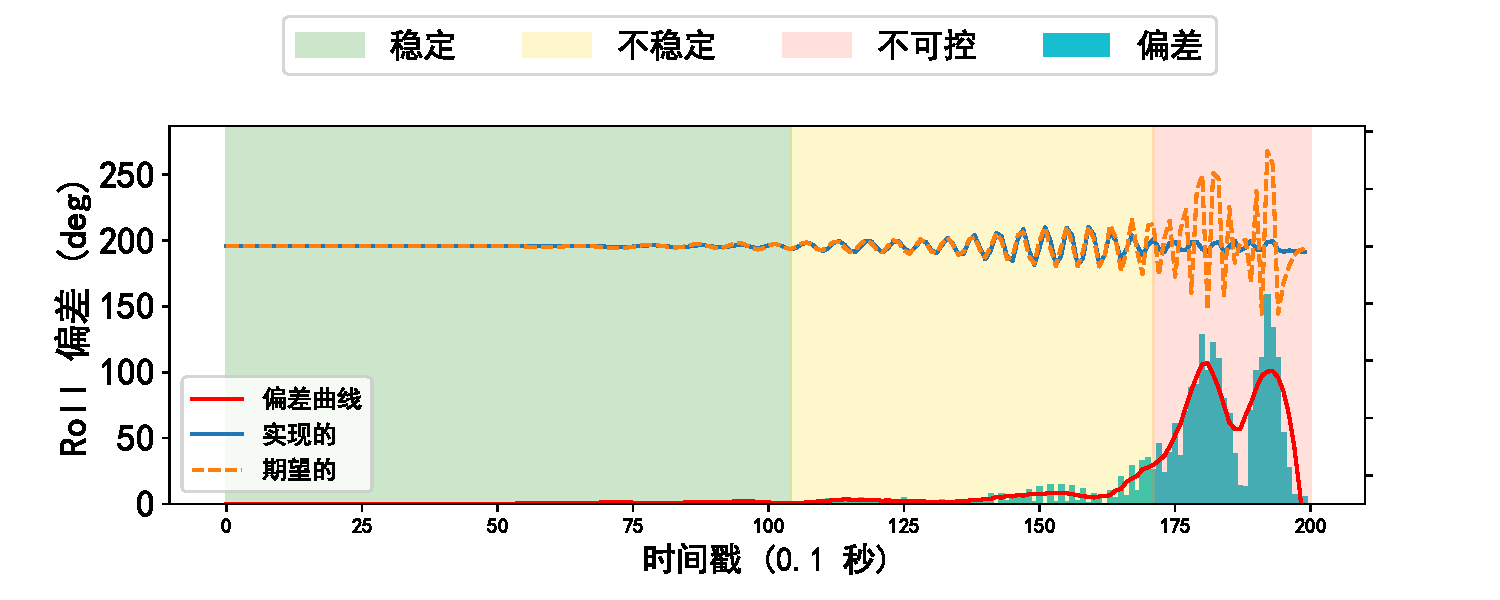
\includegraphics[width=0.88\linewidth]{fig/fix/unstable/frozen_states_roll.pdf} \\  
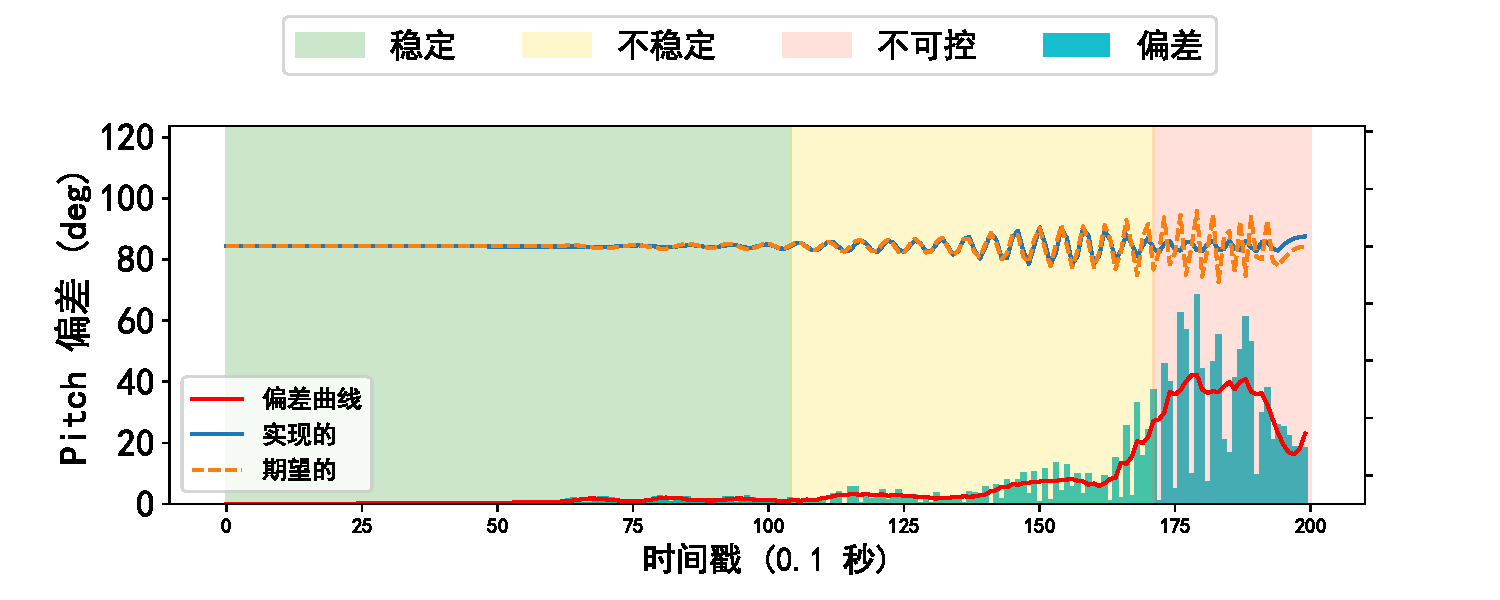
\includegraphics[width=0.88\linewidth]{fig/fix/unstable/frozen_states_pitch.pdf} \\
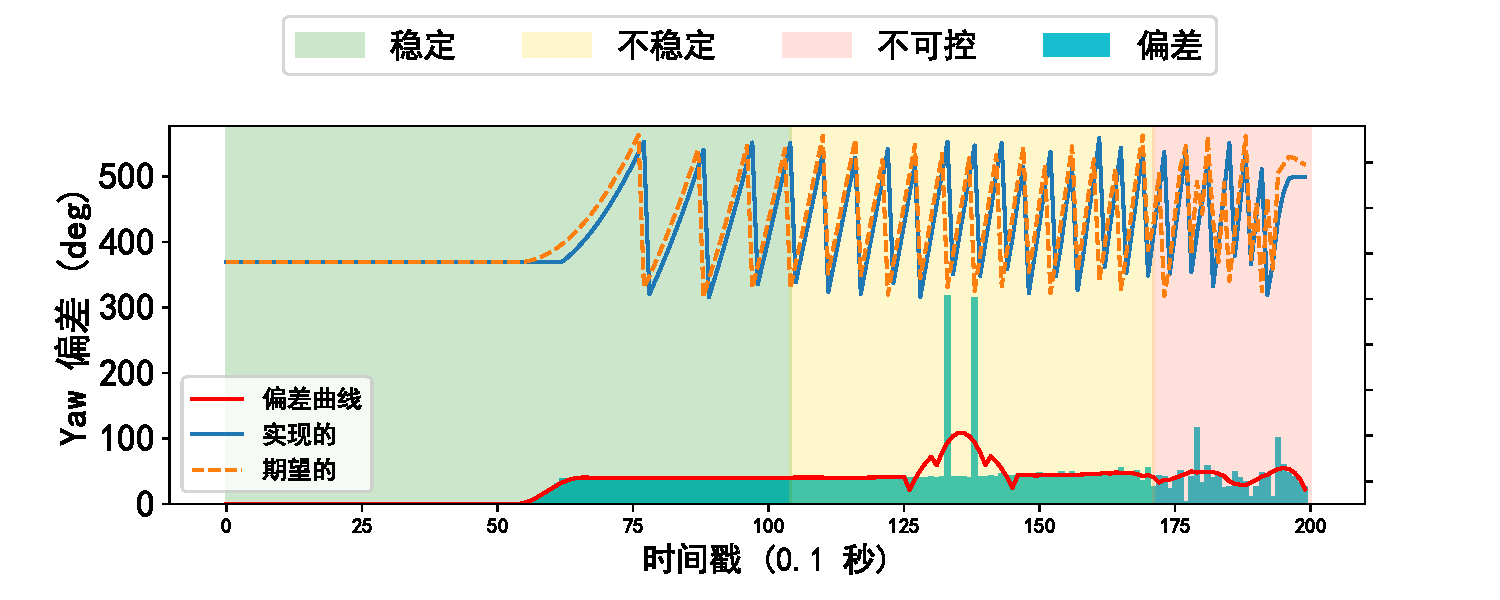
\includegraphics[width=0.88\linewidth]{fig/fix/unstable/frozen_states_yaw.pdf}
}
\caption{物理状态的角度变化}
\label{fig:frozen_state}
\end{figure}
根据偏差柱状图的观察结果,手动定义其三个阶段为:
\begin{itemize}
\item \textbf{0 to 10.3秒 (稳定)} 
在使用正常配置进行飞行任务时,无人机保持了稳定性。其每个状态下的现实的滚转、俯仰和偏航都符合预期,从图中也可以观察到,该阶段的偏差值都非常小,几乎可以忽略。


\item \textbf{10.4s to 17.1秒 (不稳定)}
无人机接收到不正确的配置后,其飞行姿态逐渐变得不稳定,表现出摇摆并且该阶段的偏差是逐渐增大的。
在这一阶段,无人机仍然按照正确的轨迹飞行,因为其自身的控制算法任然尝试矫正其飞行,但是已经出现了潜在的不稳定因素。
由于无人机仍然遵循着既定的飞行计划,这时仍然可以通过发送有效配置来矫正不稳定的物理状态,从而消除不利影响。


\item \textbf{17.2秒 之后 (不可控)}
随着这种不稳定因素的叠加,无人机已经无法正确的维持自身的飞行稳定,从而造成了较大的偏差。
图中显示的偏差也说明了混乱的状态。
飞行控制程序也检测到了不稳定状态,因为出现了明显的不稳定性和偏差,并报告了错误警告,且当前的飞行状态已经很难通过用户指令恢复正常。

\end{itemize}

观察结果表明,不正正确配置当在不稳定阶段中被发现并消除,这样无人机才能有恢复的可能。
因此,本节设计工具的目标是探索不稳定阶段,然后进行控制参数矫正,以矫正不稳定状态。



\subsection{在线矫正的特点}
对于范围规范错误,上一章的解决方案是在飞行前尽可能能让用户在安全的范围内选择参数配置。
但是相应的结果表明,这不能完全的杜绝所有的不正确配置的情况,尤其实在有外部攻击可能性的情况下,用户更加却反应对措施。
因此,在有上一章节的范围指南的情况下,依旧需要引入动态的飞行矫正方案,能够高效的解决飞行中突发攻击的防御场景,全方位的保障飞行安全。

而飞行中对参数进行矫正有以下挑战。

\begin{itemize}
    \item \textbf{挑战 1:不同飞控程序中控制参数设计及参数取值范围不一致。}
    由于缺乏统一的行业标准,制造商可以利用不同的控制参数元素将不同的功能合并到他们的飞行控制程序中。
    即使对于实现相同目标的参数元素,制造商可能会使用不同的参数名称。、
    此外,具有相同功能的参数的取值范围在不同的飞行控制程序中也可能不同。
    表~\ref{tab:fix_dis_params} 展示了两个流行的飞控程序\tool{Ardupilot}和\tool{PX4}中参数的比较。
    两个飞行控制程序都包含 2000 多个参数,但只有 249 个实现相同的功能。
    此外,每个飞行控制程序都有大约 100 个控制姿态相关控制参数,但只有 37 个(35\%)实现相同的功能。

    \begin{table}[ht]
\caption{不同控制程序中的参数(有范围限制的参数)}
\label{tab:fix_dis_params}
\centering
\begin{tabular}{c|cc}
        \toprule[1.5pt]
        ~ & \tool{Ardupilot} & \tool{PX4} \\
        \midrule[0.8pt]
        总计 & 2,990 & 2,407 \\
        \midrule[0.8pt]
        \makecell[c]{完全相同} & \multicolumn{2}{c}{66}  \\

        \makecell[c]{功能和范围相同} & \multicolumn{2}{c}{16}  \\

        \makecell[c]{仅功能相同} & \multicolumn{2}{c}{249}  \\
        
        \midrule[1.5pt]

        姿态相关的参数 & 105(3.5\%) & 101(3.5\%) \\
        \midrule[0.8pt]
         \makecell[c]{完全相同} & \multicolumn{2}{c}{0}  \\

        \makecell[c]{功能和范围相同} & \multicolumn{2}{c}{0}  \\

        \makecell[c]{仅功能相同} & \multicolumn{2}{c}{37}  \\
        
        
        \bottomrule[1.5pt]
\end{tabular}
\end{table}
   
    \item \textbf{挑战 2:控制参数之间相互依赖复杂,实时选择合适的配置较为困难。}
    控制参数的相互依赖性错综复杂地交织在一起,因为无人机中的所有组件都具有较高的关联性~\cite{ding2023get}。
    因此,有效管理这些依赖关系对于正确设置配置和消除不正确导致的不稳定至关重要。
    但是,与控制参数相关的初始化和范围检查代码通常是独立实现的,并且不考虑参数之间的相互依赖性。
    与起飞前测试的方式不同的是,在飞行过程中几乎没有可能考虑控制参数的如此复杂的值组合。
    因此测试所有组合(即配置)是不可行的。
    
    
    \item \textbf{挑战 3:配置受到不确定性执行环境的影响,产生意想不到的副作用。}
    由于执行环境的开放性,由配置产生的飞行状态的性能可能与预期的不同。
    虽然一些研究方法试图通过建立先验知识来描述潜在的执行条件来处理这种环境不确定性,尽管可以正确实施和设置与姿态相关的控制参数,很难估计现实中无人机飞行时的环境变化及其对姿态相关参数的影响。
     
\end{itemize}

\subsection{解决方案}
基于上述研究,稳健的控制参数矫正机制必须满足以下要求:

\begin{itemize}
\item \textbf{即时控制参数矫正:}
通过先前状态变化的样例可以发现大多数威胁首先导致无人机进入不稳定(但并非无法控制)的物理状态。
对此,如果发现不稳定的物理状态并及时生成新的控制参数配置,飞控程序就有足够的时间做出响应并重新驾驶无人机进入预期状态。
此外,多项研究~\cite{choi2020cyber,zhou2022doublestar}表明,某些入侵方法会持续攻击无人机,因此,不是在无人机起飞之前进行各种检查或者限制,而是在整个飞行过程中,矫正也应该持续进行,以保护控制参数 。


\item 
\textbf{自适应矫正:}
由于许多无人机不提供其控制程序的源代码且参数的名称和功能没有统一的规则,因此应用替代控制算法~\cite{choi2020software,dash2021pid}来增强原始飞行系统是不可行的。
可行的是,现在大多数无人机都提供配置调整接口,并且制造商通常会发布相应的手册来提供帮助。
因此,利用原生的控制参数配置接口来帮助无人机调整物理状态,相比需要重新编译原始无人机系统的解决方案要方便得多。
此外,由于这种设计使用的是无人机自身提供的内部机制,因此可以应用到不同的飞行控制程序中。

\end{itemize}

\section{方案}
本节介绍\nyctea 的设计和实现。首先介绍其架构的概述,然后详细讨论。

\subsection{概览}

\begin{figure*}[htb]
  \centering
    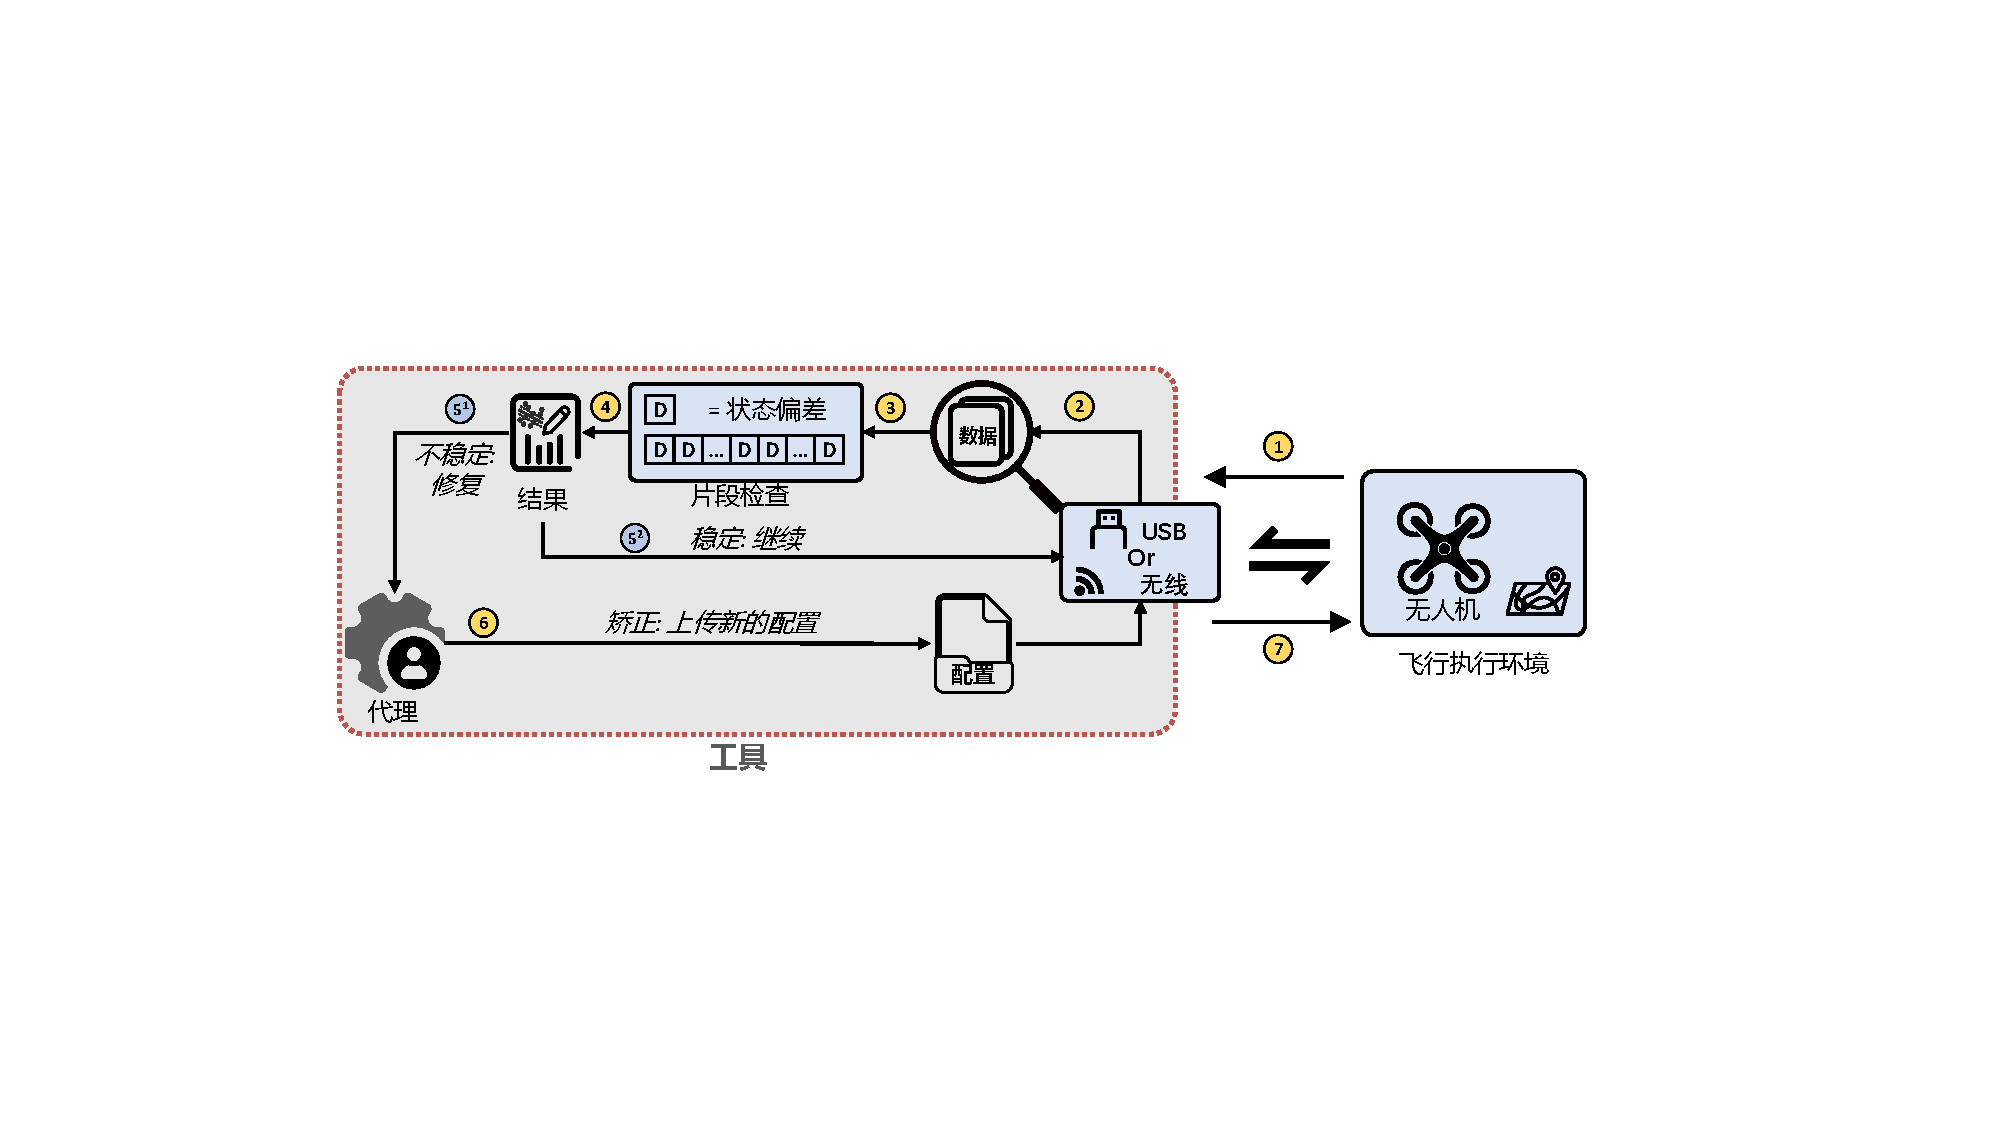
\includegraphics[width=\linewidth]{fig//fix/overview_fix.pdf}
\caption{\nyctea 架构概览}
\label{fig:fix_overview} 
\end{figure*}

\nyctea 的架构如图~\ref{fig:fix_overview} 所示。
\nyctea 利用无线或USB与无人机连接。 (\circled{1})。
它使用动态监控方法,利用段状态来跟踪无人机物理状态的变化(\circled{2}\circled{3})。
一旦获得段,\nyctea 就会计算段中的期望状态和实现状态之间的偏差 (\circled{4})。
如果所有状态偏差的总和低于预定义的阈值,\nyctea 会继续监视下一段 (\circled{$5^2$})。
否则,\nyctea 认为无人机具有不稳定的物理状态 (\circled{$5^1$}),并通过智能体模型创建配置来调整其飞行 (\circled{$6$})。
该过程是迭代的,\nyctea 捕获段偏差并实时矫正无人机。
下面首解释如何在\emph{飞行与校正建模}中对校正问题进行建模,如何进行\emph{智能体训练},以及在\emph{实时矫正}中的应用。


\subsection{飞行与校正建模}
矫正不稳定物理状态的问题可以从飞行物理稳定性的优化问题转换为奖励最大化问题,也就是什么样的配置能使当前状态获得最大的奖励(稳定性)。

\subsubsection{智能体状态}
为了有效地解决这个问题,本方案需要一个能够准确表示当前不稳定物理状态的智能体状态描述。 
该描述应捕获已实现的飞行状态与期望状态之间的偏差,使智能体能够生成适当的动作(即配置)作为响应。
考虑到不稳定状态的性质,智能体状态描述需要同时考虑无人机的物理状态和相应的传感器测量数据。

无人机在飞行过程中实时生成飞行日志数据。
\nyctea 通过生成片段来预处理飞行数据以供进一步分析。
在每个时间戳$t$,\nyctea 分别检索物理飞行状态$a_t$、期望飞行状态$a'_t$。
由于无人机可以完成360度翻滚, 此处物理和期望的飞行状态值被记录为基于弧度的。
此外,\nyctea 从陀螺仪和加速度计测量中获取相应的传感器数据 $e_t$。
在时间戳 $t$ 捕获的每个航班数据可以用一个三元组表示,即 $s_t = \{a_t, a'_t, e_t\}$。
\nyctea 收集连续的飞行数据形成一段$S$来探索偏差变化。
一个段,记录从时间戳$t$收集的数据,表示如下:
\begin{equation}
    S_t = \{s_j~|~j \in [t, t+m_{3}-1]\}
\end{equation}
其中$m_{3}$是段的长度。

\subsubsection{不稳定监测}
对于分段,系统通过检查期望状态和物理状态之间的分段偏差是否超出可接受的范围来监控无人机的不稳定性。
$S_t$ 段中的物理状态和期望状态为:
\begin{equation}
\begin{aligned}
    A_t = \{~a_j~|~j \in [t, t+m-1]~\}\\
    A'_t = \{~a'_j~|~j \in [t, t+m-1]~\}
\end{aligned}
\end{equation}
\nyctea 首先计算每个物理飞行状态与其相应的期望飞行状态之间的一范数:
\begin{equation}
d_j = ~\Vert~a_j - a'_j~\Vert, ~j \in [t, t+m-1]
\end{equation}
然后,\nyctea 通过对各个偏差 $Dv_t=\sum_{t}^{t+m-1}{d_j}$ 求和来计算分段偏差值 $Dv_t$。
如果 $Dv_i$ 大于阈值 $TH$,则 \nyctea 识别出不稳定状态(章节~\ref{subsec:fix_th_decided} 介绍了实验设置用于此阈值的值的方法),然后激活状态矫正器模块。否则,\nyctea 继续捕获并分析下一段。

\subsection{状态矫正}
当报告不稳定时,系统将段作为输入,并利用基于配置的控制方案来纠正状态以消除不稳定性。
整改过程使用预先训练的学习智能体,逐渐消除不稳定因素。

\subsubsection{动作空间}  
\nyctea 的目标是给出适当的动作(配置)来调整当前无人机来保持稳定。
动作空间可以定义为智能体可以采取的所有可能动作的集合。
对于本问题,动作空间$\mathbb{C}$被定义为所有可能的参数组合的集合,这些组合受到官方指南和规范的约束。
具体的动作(配置)$c$如下所示:
\begin{equation}
    c = \{~p'_1, p'_2, ..., p'_{n3}~\}, c \in \mathbb{C}
\end{equation}
其中 $p'$ 是新参数值,$n$ 是配置中的参数数量。

\subsubsection{动作模型训练}
\nyctea 训练一个参与者模型来生成用于纠正的配置,并根据制定的奖励函数增强模型。
训练执行了一架配置错误的无人机来完成飞行任务~\tool{AVC2013}~\cite{avc}。
在训练之前,\nyctea 利用之前的模糊测试工具,生成大量的不正确配置用于训练。
在每次执行最初使用其默认配置启动飞行控制程序。
然后在第一个航路点上传不正确配置。
随后启动\nyctea 中的智能体来进行矫正的修复。
它收集矫正经验并更新智能体,在后续检测到不稳定阶段时生成适当的配置。
\nyctea 通过深度强化学习策略\tool{(Deep Deterministic Policy Gradient,DDPG)}~\cite{lillicrap2015continuous}来实现该目标,详细步骤见算法~\ref{alg:fix_system}。

\SetAlFnt{\small}
\begin{algorithm}[htb]
\caption{训练流程}\label{alg:fix_system}
 \LinesNumbered
 \KwIn{
训练批量尺寸 $N$, 软更新因子 $\tau$, 贴现系数 $\gamma$,
 不正确配置集 $ICs$, 偏差阈值 $TH$
 \;
 }
 初始Critic网络 $Q(\cdot)$, $Q'(\cdot)$\ 包含权重 $\theta^{Q}$, $\theta^{Q'}$\;
 初始Actor网络 $\mu(\cdot)$ and $\mu'(\cdot)$ 包含权重 $\theta^{\mu}$, $\theta^{\mu'}$\;
 最初, $\theta^{Q'} \gets \theta^{Q}$, $\theta^{\mu'} \gets \theta^{\mu}$\;
 重播缓冲区 $R$\;
 
\For{$ic_{k}$ in $ICs$}{
    初始化飞行场景 $ic_{k}$ 并启动\;
    \For{时间戳 $i$ in  执行($ic_{k}$)}{
      观察一个片段 $S_t$\;
      计算偏差 $Dv_t$\;
      \If{$Dv_t < TH$}{
        continue;
      }

      
      选择动作 $c_t \gets \mu(S_t)$\;
      $S_{next}$, $r_t$ $\gets$ 执行动作 $c_t$\;
      存储元组 $(S_t, c_t, r_t, S_{next})$ in $R$\;
    
      
      \If{$length(R) < N$}{
        continue;
      }
      随机批量 $N$ 个转换元组 $(S_j, c_j, r_j, S_{(j,next)}), j \in N$ from $R$\;
    
      计算 $y_j = r_t + \gamma Q'(r_j, \mu'(S_{(j,next)})$\
      
      通过最小化损失来更新批评家 (\ref{eq:loss})\;
      %$$L = \frac{1}{N}\sum_{j}(y_j - Q(S_j, c_j))^2$$\

      使用采样的策略梯度更新参与者策略 (\ref{eq:policy})\;

      % $$\nabla_{\theta^{\mu}} \approx \frac{1}{N} \sum_{j}\nabla_{c}Q(S,c)\mid_{S=S_j, c=\mu(S_j)}\nabla_{\theta^{\mu}}\mu(S)\mid_{S_j}$$

      更新网络 (\ref{eq:sigma})\;
      % $$\theta^{Q'} \gets \tau \theta^{Q} + (1-\tau)\theta^{Q'}$$
      % $$\theta^{\mu'} \gets \tau \theta^{\mu} + (1-\tau)\theta^{\mu'}$$
      
     }
}

 
\end{algorithm}


最开始,\nyctea 设置了一些初始化因素,包括训练批量大小$N$、模型软更新因子 $\tau$、学习折扣因子 $\gamma$、偏差值阈值 $TH$(将在章节~\ref{subsec:fix_th_decided}中决定)和重播缓冲区$R$。
\nyctea 还初始化Critic网络$Q(\cdot)$、$Q'(\cdot)$ 以及权重 $\theta^{Q}$、$\theta^{Q'}$\ 和Actor网络 $\mu (\cdot)$ 和 $\mu'(\cdot)$ 的权重为 $\theta^{\mu}$、$\theta^{\mu'}$。
最初的$\theta^{Q'}$和$\theta^{\mu'}$等于$\theta^{Q}$和$\theta^{\mu}$。

随后,应用生成大量的不正确配置集$IC$来进行训练。
\nyctea 发起启动飞行测试,然后在第一个航点上传一个不正确配置,它监视飞行日志数据(即姿态状态和传感器数据)并捕获段$S_t$数据(第 8 行)。
\nyctea 计算偏差值 $Dv_t$(第 9 行)。
如果偏差值低于阈值 $TH$,则 \nyctea 继续并捕获下一段。
否则,\nyctea 将这段 $S_t$输入到Actor网络$\mu(S_t)$中并获得一个动作(配置)$c_t$(第 13 行)。
随后,\nyctea 用这个新配置上传至无人机,观察下一段$S_{next}$,使用章节~\ref{subsec:fix_reward}中的方法计算奖励$r_t$(第 14 行)。
这一系列操作生成的元组$(S_t, c_t, r_t, S_{next})$将存储在重播缓冲区$R$中(第 15 行)。
如果重放缓冲区的大小超过设定的训练批量尺寸大小,\nyctea 会从历史经验中学习并相应地更新模型权重(第 19 到 23 行)。
具体而言,\nyctea 随机采样$N$个转换元组,每个元组为:
\begin{equation}
    (S_j, c_j, r_j, S_{(j,next)}), j \in [1, N]
\end{equation}
\nyctea 随后计算:
\begin{equation}
    y_j = r_t + \gamma Q'(r_j, \mu'(S_{(j,next)})
\end{equation}
\nyctea 通过最小化损失来更新Critic:
\begin{equation}\label{eq:loss}
    L = \frac{1}{N}\sum_{j}(y_j - Q(S_j, c_j))^2
\end{equation}
并使用采样的策略梯度更新参与者策略:
\begin{equation}\label{eq:policy}
    \nabla_{\mu} \approx \frac{1}{N} \sum_{j}\nabla_{c}Q(S,c)\mid_{S=S_j, d=\mu(S_j)}\nabla_{\theta^{\mu}}\mu(S)\mid_{S_j}
\end{equation}
经过一轮策略更新后,Actor和Critic网络权重被软更新:
\begin{equation}\label{eq:sigma}
    \begin{aligned}
        \theta^{Q'} = \tau \theta^{Q} + (1-\tau)\theta^{Q'} \\
        \theta^{\mu'} = \tau \theta^{\mu} + (1-\tau)\theta^{\mu'}
    \end{aligned}
\end{equation}

其中特殊的情况是,如果无人机在飞行过程中触发严重不稳定或成功着陆,任务将重新开始,但重播缓冲区将保留。
一旦无人机能够连续三次矫正当前的不正确配置(无人机成功完成任务),训练就会进入其他实验攻击场景。
最后,在学习过程结束时,使用智能体的Actor网络 $\mu$ 来生成校正。


\subsubsection{奖励函数}\label{subsec:fix_reward}
对于智能体状态 $S_t$,\nyctea 会计算偏差值$Dv_t$。
然后通过智能体的Actor$\mu(\cdot)$来根据此状态生成一个操作(即配置$c_t$)并将其上传到无人机:
\begin{equation}
    c_t = \mu(S_t)
\end{equation}
\nyctea 观察下一个智能体状态$S_{next}$作为此操作的结果,并以相同的方式计算下一个偏差值$Dv_{next}$。
偏差变化$Dc$计算为先前偏差值和新偏差值之间的差:
\begin{equation}
    Dc_t = Dv_{next} - Dv_t
\end{equation}
根据 $Dc_t$ 值,\nyctea 采用不同的策略给予奖励:

\begin{itemize}
    \item \textbf{正值:} 如果偏差值$Dv_t>0$, 此训练过程并不会直接使用该偏差值作为奖励。
    \nyctea 设计的整体目标是生成的配置需要尽可能的将一个无人机飞行状态从一个较大的偏差减少到较小的偏差,也就是从不稳定变化到更稳定。
    即使中间出现较大额偏差缩减,但是缩减后的偏差没有保持一个较小的值的话,也不应获得较大的奖励。
    而通过矫正配置后的偏差$S_{next}$越接近于零,则配置会应该收到更大的奖励。
    相反,即使$Dc_t$有较大的偏差变化,但是下一个偏差值$Dv_{next}$不接近于零(足够稳定),配置也不应获得更大的奖励。
    除此之外,智能体可能会为了追求高奖励而生成过于极端的配置,例如允许无人机在飞行中悬停并达到较小的下一个偏差值$Dv_{next}$,这会导致无人机无法继续完成任务,与修复目标本身相违背。
    为了防止这种情况,\nyctea 将最小值$Dv_{next}$设置为1,即 $max(1, Dv_{next})$并将$Dc_t$乘以一个加速比例$acc_t$。
    该加速比例为矫正配置造成给下一时刻$S_{next}$中的平均加速度。
    在该加速度比例的影响下,如果矫正配置是的无人机的动作变化太小,则相应的奖励权重将会变小。
    总体上讲,所设计的正值奖励计算方式如下:
    \begin{equation}
        r_t = \frac{Dc_t * acc_t}{max(1, Dv_{next})}
    \end{equation}

    下面将通过一些例子说正值奖励的处理过程。
    假设配置将偏差从$80$减少到$20$,造成的下一个时刻数据片段的加速比例为$1.2$。
    此时前后两个片段数据产生的偏差变化为$60$。
    虽然这个偏差减少量不算少,但是由于下所造成的片段状态(偏差为$20$)仍然不稳定。
    \nyctea 认为这种配置有一些积极作用,但不足以获得更大的奖励。
    因此,它只能获得$\frac{60*1.2}{20}=3.6$奖励。
    假设另一种配置以$0.8$的加速比例将偏差从$20$减少到$1$,则它可以获得$\frac{20*0.8}{1}=16$的更高奖励,因为作为其后续片段(偏差值为$1$)更稳定。
    令一种极端的情况是,假设配置将偏差从$80$减少到$20$,但加速比例为$0.1$,也就是以为着无人机几乎停止移动。
    它只收到$\frac{60*0.1}{20}=0.3$奖励。

    \item \textbf{负值:} 如果偏差值$Dv_t<0$, 训练过程会对该配置进行惩罚。
    即使智能体生成的配置不能充分减轻偏差,该配置也不应该进一步加剧不稳定性,也就是增加偏差。
    因此,如果偏差值$Dc_t$为负,则\nyctea 直接使用偏差变化值$Dc_t$作为奖励。
    例如,假设配置将偏差值从$20$加剧到了$30$,智能体将收到$30-20 = -10$的奖励。
    

    \item \textbf{严重不稳定或特殊情况:}     
    如果配置直接触发失控(例如,坠毁、推力损失和无法控制的飞行的轨迹偏差),\nyctea 将负面奖励加倍作为惩罚形式。
    也就是说,即使该配置稳定了无人机,但导致了严重的事件,例如稳定后方向错误(轨迹偏差),也不会得到积极的奖励。
    
\end{itemize}


\subsection{实时矫正}
一旦进入失控阶段,无人机可能会出现极大的偏差,无法矫正飞行。
为了防止这种情况发生,\nyctea 会检测不稳定的物理状态并启动适当的配置。
\nyctea 不断捕获飞行段数据$S$并计算偏差值$Dv$。
参考检测阈值$TH$,如果偏差值超过阈值,则\nyctea 将使用不稳定标签标记捕获的片段。
然后,\nyctea 将当前段$S$输入到智能体中,并获取用于更新无人机的新配置。
如果下一个观察到的偏差仍然超过阈值,则继续矫正。

\section{实验结果及分析}

本章节通过检测精度和矫正成功率方面评估\nyctea 的性能,同时还分析误报和时间消耗。
\begin{itemize}
 
\item \textbf{研究问题1 识别准确率:} \nyctea 能否实时有效识别不稳定因素?

\item \textbf{研究问题2 矫正性能:} \nyctea 能否消除不稳定因素,成功防范潜在威胁? 涉及的控制参数数量是否影响整改成功率?

\item \textbf{研究问题3 时间消耗:}\nyctea 需要多长时间才能生成配置并最终消除不稳定因素?

\end{itemize}
\subsection{实验准备}

\subsubsection{实验设定}

\begin{itemize}
    \item \textbf{实验程序:}
实验主要在两个流行的飞行控制程序 \tool{ArduPilot} (4.2.0)~\cite{ardupilot} 和 \tool{PX4} (1.13)~\cite{px4} 上测试了 \nyctea。
此处的实现使用 \tool{Mavlink}~\cite{mavlink} 将 \nyctea 与 \tool{Ardupilot} 和 \tool{PX4} 连接,并调用第三方包的函数\tool{Pymavlink}~\cite{pymavlink} 用于数据捕获和配置上传。
由于实验硬件以10Hz将内存数据写入闪存,因此采用统一的采样率10Hz,也就是数据采集间隔是$0.1s$。
根据手动测试,飞行控制程序通常需要两秒以上才能对不正确做出反应。
因此,本实验中的片段通过连续捕获两秒的数据形成。
鉴于 \nyctea 每 $0.1s$ 捕获一次飞行数据,每轮分析涉及一个大小为$20$的数据片段。
关于智能体设置,本实验将缓冲区的最大容量设置为 $20,000$,软更新因子为 $0.02$,折扣因子为 $0.99$,批量大小为 $64$。
Actor和Critic的网络具有相同的网络结构,其中包含三个隐藏大小为256的线性层。

\item \textbf{测试设备:}
由于不稳定可能会导致无人机遭受物理损坏以及涉及行人的潜在事故的风险,实验使用模拟器进行了大部分实验。
使用配备\tool{Ardupilot}的\tool{APM}和配备\tool{PX4}的\tool{Jmavsim}。
对于一些导致较小风险的测试用例,实验将这些案例集成到配备\tool{Ardupilot}的物理无人机\tool{CUAV ZD550} 中,以评估工具在现实场景中的性能。

\item \textbf{参数选择:}
每个飞行控制程序由数百个参数组成,但其中只有少数参数与飞行调整和稳定性密切相关。
因此,实验根据官方手册提供的控制参数说明,选择了与角姿态和角速率相关的参数。
如表~\ref{tab:fix_param_both}所示,实验从\tool{Ardupilot}中选择了$17$参数,从\tool{PX4}选择了$11$参数。

% \begin{table}[ht]
% \small
% \caption{Parameters for experiments.}
% \label{tab:param_both}
% \centering
% \begin{tabular}{c|c}
%         \toprule[1.5pt]
%         \textbf{Ardupilot} & \textbf{PX4}\\
%         \midrule[0.8pt]
%     \makecell*[c]{PSC\_VELXY\_P\\PSC\_VELXY\_I\\PSC\_VELXY\_D\\PSC\_ACCZ\_P\\PSC\_ACCZ\_I\\ATC\_ANG\_RLL\_P\\ATC\_RAT\_RLL\_P\\ATC\_RAT\_PIT\_I\\ATC\_RAT\_RLL\_D\\ATC\_ANG\_PIT\_P\\ATC\_RAT\_PIT\_P\\ATC\_RAT\_PIT\_I\\ATC\_RAT\_PIT\_D\\ATC\_ANG\_YAW\_P\\ATC\_RAT\_YAW\_P\\ATC\_RAT\_YAW\_I\\ATC\_RAT\_YAW\_D\\} 
%     & 
%     \makecell*[c]{ MC\_ROLL\_P\\MC\_PITCH\_P\\MC\_YAW\_P\\MC\_YAW\_WEIGHT\\MPC\_XY\_P\\MPC\_Z\_P\\MC\_PITCHRATE\_P\\MC\_ROLLRATE\_P\\MC\_YAWRATE\_P\\MPC\_TILTMAX\_AIR\\MPC\_TKO\_SPEED} \\
%     \bottomrule[1.5pt]
% \end{tabular}
% \end{table}

\begin{table}[ht]
\small
\caption{实验参数}
\label{tab:fix_param_both}
\centering
\begin{tabular}{c|c|c}
\toprule[1.5pt]
\textbf{参数描述}      & \textbf{Ardupilot} & \textbf{PX4}          \\ 
\midrule[0.8pt]
Roll angle P gain         & ATC\_ANG\_RLL\_P   & MC\_ROLL\_P           \\ \hline
Pitch angle P gain        & ATC\_ANG\_PIT\_P   & MC\_PITCH\_P          \\ \hline
Yaw angle P gain          & ATC\_ANG\_YAW\_P   & MC\_YAW\_P            \\ \hline
Roll rate P gain          & ATC\_RAT\_RLL\_P   & MC\_ROLLRATE\_P       \\ \hline
Pitch rate P gain         & ATC\_RAT\_PIT\_P   & MC\_PITCHRATE\_P      \\ \hline
Yaw rate P gain           & ATC\_RAT\_YAW\_P   & MC\_YAWRATE\_P        \\ \hline
Roll rate I gain          & ATC\_RAT\_RLL\_I   &                       \\ \hline
Roll rate D gain          & ATC\_RAT\_RLL\_D   &                       \\ \hline
Pitch rate I gain         & ATC\_RAT\_PIT\_I   &                       \\ \hline
Pitch rate D gain         & ATC\_RAT\_PIT\_D   &                       \\ \hline
Yaw rate I gain           & ATC\_RAT\_YAW\_I   &                       \\ \hline
Yaw rate D gain           & ATC\_RAT\_YAW\_D   &                       \\ \hline
Velocity P gain           & PSC\_VELXY\_P      &                        \\ \hline
Velocity I gain           & PSC\_VELXY\_I      &                        \\ \hline
Velocity D gain           & PSC\_VELXY\_D      &                        \\ \hline
Acceleration P gain.      & PSC\_ACCZ\_P       &                        \\ \hline
Acceleration P gain.      & PSC\_ACCZ\_I       &                        \\ \hline
Yaw weight                &                    & MC\_YAW\_WEIGHT       \\ \hline
Horizontal error gain     &                    & MPC\_XY\_P            \\ \hline
Vertical error gain       &                    & MPC\_Z\_P             \\ \hline
Maximum tilt angle        &                    & MPC\_TILTMAX\_AIR     \\ \hline
Takeoff climb rate        &                    & MPC\_TKO\_SPEED       \\ 
\bottomrule[1.5pt]
\end{tabular}
\end{table}



       

\end{itemize}


\subsubsection{配置数据集构造}
为了评估 \nyctea 的性能,实验首先构建了一个包含安全配置和不正确配置以及相应飞行状态的配置数据集。
实验使用\tool{LGDFuzzer}~\cite{han2022control} 来探索潜在的安全配置和不正确。
然后通过将这些配置输入飞行模拟器来执行飞行任务\tool{AVC2013}~\cite{avc},这些飞行任务的第一个航路会有意地点引入不正确配置。
最后,实验过程中会使用利用 \tool{PyMavlink} 来检查每个飞行任务是否成功完成。
如果一个飞行测试中无人机顺利降落,则该测试配置被确认为 \dquote{安全}; 否则,被认为是\dquote{不正确配置}。

通过实验观察发现配置会导致飞行状态下的不同的无人机错误报告:
\begin{itemize}
\item 执行器相关错误(AR):它导致飞行控制程序报告与执行器相关的警告,例如潜在的推力损失、油门错误、偏航不平衡和碰撞。

\item 任务执行错误(ME):使飞行轨迹偏离预期路径,如轨迹偏离、飞行悬停等。

\item 系统故障保护错误(SF):导致飞控程序报告故障保护,例如EKF故障保护(位置和姿态估计系统不健康)和传感器故障保护(传感器测量值不一致)。

\end{itemize}

实验总共对\tool{Ardupilot}控制程序收集了6,545个配置,包括 1,781 个安全配置和4,764个不正确,以及对\tool{PX4}收集了4,829 个配置,其中包括 1,367 个安全配置和 3,462个不正确。
由于\nyctea 需要阈值 $TH$ 来确定无人机的稳定性,并依赖智能智能体来生成正确的配置,实验将数据集分为训练集和测试集。
训练集用于确定阈值并训练智能体,而测试集用于评估系统。
具体来说,实验分别在\tool{Ardupilot}和\tool{PX4}中随机选择了1,000个安全配置,并分别从\tool{Ardupilot}和\tool{PX4}中选择了2,785和2,228个不正确。
数据集详细信息列于表~\ref{tab:fix_unstable_env} 中。

\begin{table}[ht]
\caption{测试场景分布}
\label{tab:fix_unstable_env}
\centering
\begin{threeparttable}
\begin{tabular}{c|cccc}
        \toprule[1.5pt]
        ~ & {\makecell*[c]{安全}}  & {\makecell*[c]{执行器相关}} & {\makecell*[c]{任务执行}} &  {\makecell*[c]{系统故障保护}} \\
        
        \midrule[0.8pt]
        
        \tool{Ardupilot} & 781 & 716  & 938 & 325 \\
        
        \tool{PX4} & 367 & 316  & 798 & 120 \\
        
        \bottomrule[1.5pt]
\end{tabular}
\end{threeparttable}
\end{table}


\subsection{不稳定阈值设定}\label{subsec:fix_th_decided}
无人机飞行中出现不稳定的情况必然导致物理状态和期望状态之间出现偏差。
因此,实验使用训练数据集中的安全配置和不正确手动启动飞行执行,以确定 $TH$。
对于具有安全配置的每次飞行执行,实验随机在其飞行过程中的任意时间戳捕获片段。
而对于配置错误的飞行执行,实验在报告错误或警告后随机捕获片段。
随后,实验计算了从安全配置执行中收集的平均偏差值 $Dv_{(safe,avg)}$ 以及从不正确配置的执行中收集的平均偏差值 $Dv_{(mis, avg)}$。
最终,两者的中值被视为监测阈值 $TH$:
\begin{equation}
    TH = (Dv_{(safe,avg)} + Dv_{(mis,avg)})/2
\end{equation}

表~\ref{tab:fix_threshold} 列出了最小和最大偏差值以及阈值 $TH$。
从表中可以观察到,不论\tool{Ardupilot}还是\tool{PX4},最小和最大偏差值都表现出了显着差异,这表明设置安全和不正确时的段的数据模式非常不同。
在后续实验中,\tool{Ardupilot}相关的检测阈值设置 $TH$=$22.24$,\tool{PX4}的检测阈值设置为$TH$=$17.85$。

\begin{table}[ht]
\caption{不同类型段偏差值}
\label{tab:fix_threshold}
\centering
\begin{tabular}{c|c|ccc|c}
        \toprule[1.5pt]
        {程序} & {类型} & {最小值} & {最大值} & {均值} & $TH$ \\
        \midrule[0.8pt]
        \multirow{2}*{\tool{Ardupilot}} & 安全 & 0.03 & 17.41 & 1.73 &  \multirow{2}*{22.24}\\
        
        ~ & 错误配置 & 3.22 & 318.41 & 42.76 \\
        \midrule[0.8pt]
         \multirow{2}*{\tool{PX4}} & 安全 & 0.04 & 15.46 & 1.53 &  \multirow{2}*{17.85} \\
        
        ~ & 错误配置 & 2.41 & 305.45 & 34.18\\
    
        \bottomrule[1.5pt]
\end{tabular}
\end{table}

\subsection{工具评估}
实验利用测试数据集中2,760 个配置,包括\tool{Ardupilot} 的 781 个安全配置和 1,979 个不正确配置,以及 \tool{PX4} 的367个安全配置和1,234个不正确配置。
与之前的飞行测试类似,实验启动在第一个航路点之后发送配置。

\subsubsection{评估标准}
实验定义以下指标来准确评估检测和矫正:

\begin{itemize}
\item \textbf{识别:} 表示\nyctea 汇报的的不稳定执行的数量。

\item \textbf{错失:} 表示在无人机失去控制之前 \nyctea 未检测到的不稳定执行的数量。

\item \textbf{修正:} 是\nyctea 成功矫正报告的不稳定执行的数量,从而使无人机回到稳定的偏差范围并完成飞行任务。

\item \textbf{失败:} 表示报告的无法矫正并最终导致控制丢失的不稳定执行的数量。
\end{itemize}

\subsubsection{检测精度}
表~\ref{tab:fix_system_detection} 报告\nyctea 在检测由不正确配置引起的不稳定(即检测不正确的数量)方面的性能。
具体来说,在 \tool{Ardupilot} 中,\nyctea 成功检测到 $1,979$ 中的 $1,962$,实现了 $99.51\%$ 的 F1-Score; 在\tool{PX4}中,\nyctea 成功识别了$1,234$中的$1,219$,实现了$98.76\%$的F1-Score。


\begin{table}[ht]
\caption{不稳定执行的检测结果}
\label{tab:fix_system_detection}
\small
\centering
\begin{threeparttable}
\begin{tabular}{c|ccc|ccc}
        \toprule[1.5pt]

         &  识别 & 修正 & 错失 & Precision & Recall & F1-Score\\
        
        \midrule[0.8pt]
        
        \tool{Ardupilot} & 1,964 & 1,962 & 17& 99.89\%  & 99.14\% &  99.51\%   \\
        \tool{PX4}  & 1,222 & 1,219 & 15 &99.75\% & 98.78\% &  98.76\%  \\
        
        \bottomrule[1.5pt]
\end{tabular}
\end{threeparttable}
\end{table}

对未报告的处决进行人工检查后(\tool{Ardupilot}中的$17$个和\tool{PX4}中的$15$个),研究了\nyctea 出现检测遗漏的两种具体情况:
\begin{itemize}
\item \textbf{部分角度偏差:} 由于飞行状态是由三个坐标(即Roll、Yaw、Pitch)的值控制的。
在其中的12个例子中,存在只有一个坐标的角度值显着偏离,而其他坐标保持稳定。
在这些场景下,尽管分段偏差可能保持在可接受的范围内,但无人机仍然可能会失去控制。


\item \textbf{轻微偏差变化:} 系统依靠一定时期内的偏差变化来判断是否不稳定。
假设无人机事件通常发生在短时间内,实验在实验中每两秒收集一次飞行数据。
然而, 实验观察到,在有20个实例中,无人机每两秒仅出现轻微偏差; 因此,相应的部分被认为是稳定的。
\end{itemize}

此外,实验手动检查了五个被错误报告为\dquote{不稳定}的稳定执行。
实验发现这些执行在特定时间戳处的转动角度有明显的变化,导致段偏差值显着增加。
不过,此类误报不会影响后续飞行,因为整流器生成的配置不会对无人机造成不利影响。


\subsubsection{矫正成效}
考虑到所识别的不稳定性,系统应用智能体迭代地生成配置并将配置发送到飞行控制程序以消除不稳定性。

\begin{itemize}
    \item \textbf{矫正成功率:}
表~\ref{tab:fix_repair}显示了矫正的结果。
在表中,
     \textbf{ANC} 表示成功消除不稳定而发送的配置的平均数量。
在 \tool{Ardupilot} 中,
     \nyctea 在已识别的 $1,962$ 中成功矫正了 $1,784$ 不稳定执行,其中 AR 导致的 $637$、ME 导致的 $857$、SF 导致的 $290$,成功率达到 $90.74\%$。
在 \tool{PX4} 中,
     \nyctea 在检测到的 $1,219$ 中成功矫正了 $1,080$ 不稳定执行,其中 AR 导致的 $280$、ME 导致的 $694$、SF 导致的$106$,成功率达到 $89.49\%$。

\begin{table}[ht]
\caption{\nyctea 的整改结果}
\label{tab:fix_repair}
\centering
\begin{threeparttable}
\begin{tabular}{c|c|ccc}
        \toprule[1.5pt]
        ~ & 错误类型 &  整改 (成功率) &  失败 & ANC \\
        
        \midrule[0.8pt]
        
        \multirow{4}{*}{\tool{Ardupilot}} & 总计  &  1,784 (90.74\%)  & 178 & 4.32 \\
        \cmidrule{2-5}
        ~ & 执行器相关  &  637 (89.46\%)  & 75 & 4.43 \\
        
        ~ & 任务执行 & 857 (92.15\%)  & 73 & 4.23 \\

        ~ & 系统故障保护  & 290  (90.62\%)    & 30 & 4.30 \\
    
        
        \midrule[0.8pt]
        
         \multirow{4}{*}{\tool{PX4}} & 总计 & 1,080 (89.45\%)   &  139  & 4.57 \\
         \cmidrule{2-5}
         ~ & 执行器相关 & 280 (90.03\%)   &  31  & 4.55 \\

        ~ & 任务执行  & 694 (87.73\%)     & 97 & 4.54 \\

        ~ & 系统故障保护  & 106 (90.59\%)    & 11  & 4.62 \\
        
        \bottomrule[1.5pt]
\end{tabular}
\end{threeparttable}
\end{table}

通过对所有失败案例的人工分析,实验发现主要原因是矫正的时间时间选择。
如果从识别不正确到无人机失去控制之间的时间间隔太短,\nyctea 无法生成足够的配置来消除不稳定。
对于162个失败实例,\nyctea 报告不稳定的时间有点晚(几乎达到了不可控的状态),导致矫正时间不够。
然后实验将阈值 $TH$ 修改为较低的值,这些失败的实例可以成功矫正。
然而,较低的阈值 $TH$ 可能会通过将大量\dquote{稳定}执行报告为\dquote{不稳定}从而导致较高的误报,进一步频繁触发状态矫正模块。
尽管矫正稳定状态不会损害原来的飞行,这将浪费大量时间,并有可能忽视这一时期真正的不稳定。
因此,实验仍然选择能够正确识别最不稳定的$TH$。
分析矫正生成的配置总数后,\nyctea  在 \tool{Ardupilot} 和 \tool{PX4} 中为每个不稳定的飞行执行平均分别生成 4.32 和 4.57 个配置。


     \item \textbf{参数数量的影响:}
除了使用表~\ref{tab:fix_param_both} 中列出的所选控制参数来评估\nyctea  的矫正效果之外,实验还评估了控制参数的数量是否会影响矫正的成功率。
实验分别从\tool{Ardupilot}中选择2、4、8、12和17个控制参数,从\tool{PX4}中选择2、4、8、11。
与之前的实验类似,实验生成了与这些控制参数相关的不正确,并利用这些不正确执行了飞行任务。
表~\ref{tab:fix_rate_diff_param} 显示了涉及不同数量的控制参数时的校正结果。
控制参数的数量会对整流性能产生负面影响,当参数数量增加时,成功率往往会降低。
但系统仍能保持矫正成功率超过85\%。

\begin{table}[hbt]
\caption{不同参数数量错误配置的系统性能}
\label{tab:fix_rate_diff_param}
\centering
\begin{threeparttable}
\begin{tabular}{c|ccccc}
        \toprule[1.5pt]
        \textbf{错误配置更改的参数数量\# } & \textbf{2\#} & \textbf{4\#} & \textbf{8\#} & \textbf{12 or 11\#} & \textbf{17\#} \\
        
        \midrule[0.8pt]
        
        \tool{Ardupilot} & $\frac{4/4}{100\%}$ & $\frac{16/16}{100\%}$  & $\frac{13/13}{100\%}$ & $\frac{390/430}{90.7\%}$ & $\frac{1047/1184}{88.4\%}$ \\

        \midrule[0.8pt]
        
        \tool{PX4} & $\frac{4/4}{100\%}$ & $\frac{22/24}{91.6\%}$   & $\frac{69/74}{93.24\%}$  & $\frac{392/459}{85.4\%}$ & - \\
        
        \bottomrule[1.5pt]
\end{tabular}
\begin{tablenotes}
\item \textbf{*} 每个元素为 (整改/总体)/成功率
\end{tablenotes}
\end{threeparttable}
\end{table}


    \item \textbf{配置矫正统计:}
以\tool{Ardupilot}为例,实验在图~\ref{fig:fix_distribution}记录了生成配置的分布。
该图表明,在大多数情况下(84.66\%),\nyctea  可以使用六个生成的配置成功消除每个不稳定的执行。

\begin{figure}[htb]
\centering{
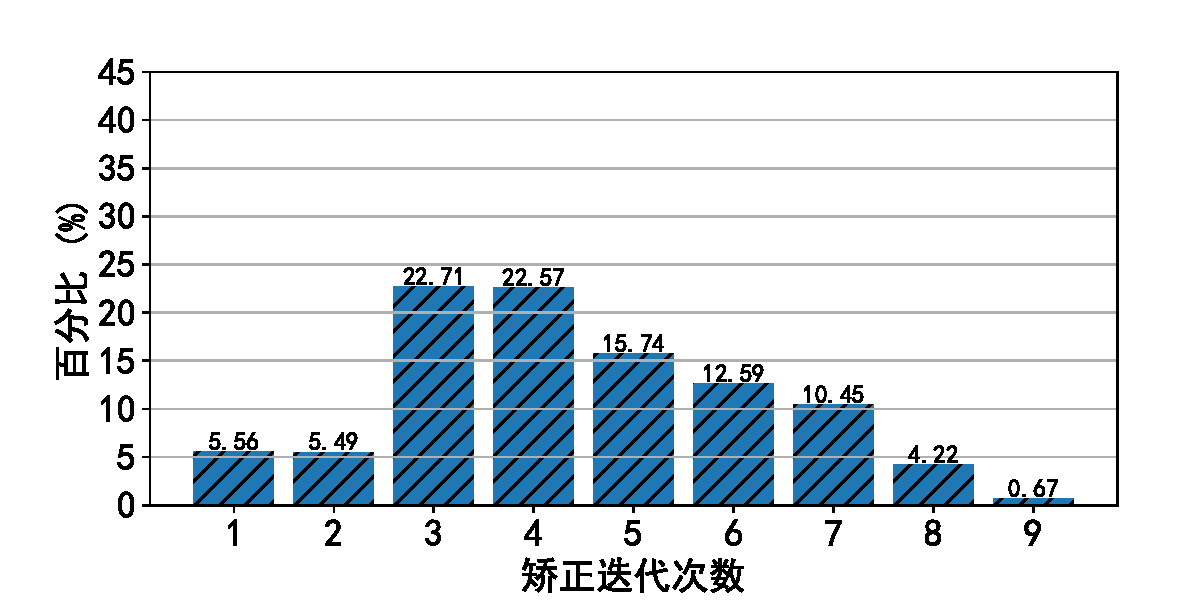
\includegraphics[width=0.95\linewidth]{fig/fix/distribution.pdf}}
\caption{成功消除不稳定因素的配置数量分布}
\label{fig:fix_distribution}
\end{figure}

\end{itemize}


\subsection{时间消耗}
实验通过分别计算训练智能体和缓解不稳定状态的时间成本来评估系统的效率。

\begin{itemize}
    \item \textbf{智能体训练.}
在智能体的训练过程中,\nyctea 消耗了 $22$ 小时从所有的不正确配置的训练集中学习修复经验。 
由于模型训练成本是一次性成本,因此 $22$ 小时是可以接受的时间成本。

    \item \textbf{状态矫正.}
实验单独评估了生成每个配置的时间消耗。
实验在 \tool{Ardupilot} 和 \tool{PX4} 中各自运智能体 500 次来创建配置。
由于模型的网络架构一直,因此两种智能体生成一种配置平均花费为 0.12ms。

\end{itemize}

    

\subsection{研究比较}
此节将 \nyctea 与其他最先进的方法(表~\ref{tab:cmp_other}) 一起讨论,这些方法也可以识别或修复影响无人机稳定性的问题。
用于解决无人机系统不稳定性的方法从两个角度解决该问题:内部错误处理和外部攻击。
内部错误处理是指由于配置错误、控制逻辑问题或安全逻辑问题等事件导致无人机不稳定的问题。
外部攻击是指由恶意活动引起的问题,例如配置攻击、传感器攻击或测量欺骗。
而用于解决无人机系统不稳定性的方法可分为三类:补丁、限制和冗余。
补丁方法涉及使用新补丁更新代码、配置、动态调整这几种方法以减少不稳定性。
限制方法利用严格的限制条件来最大程度地减少不稳定发生的可能性。
冗余方法采用额外软模块,当无人机变得不稳定时,这些模块会成为冗余控制,接管当前飞行控制系统以确保系统继续有效运行。

\begin{table*}[tb]
\caption{与最先进研究的比较}
\label{tab:cmp_other}
\centering
\begin{threeparttable}
\begin{tabular}{c|ccccccc}
        \toprule[1.5pt]
    
           & {问题源} & {修复手段} & {\makecell*[c]{在线 \\ 支持}} & {\makecell*[c]{需要 \\ 预训练}}  &  {\makecell*[c]{彻底 \\ 修复}} &{\makecell*[c]{无代码 \\ 插入} }  & {\makecell*[c]{无任务 \\ 限制} } \\
        \midrule[0.8pt]
        
          \nyctea & 内与外 & 补丁 & \ding{51} & \ding{51}  & \ding{55} & \ding{51} &  \ding{51}  \\

          \tool{LGDFuzzr}~\cite{han2022control} & 内与外 & 限制 & \ding{55} & \ding{51} & \ding{55}  & \ding{51} &  \ding{55} \\

          \tool{RVFuzzr}~\cite{rvfuzzer} & 内与外 & 限制 & \ding{55} & \ding{51} & \ding{55} & \ding{51} &  \ding{55}  \\

          \tool{DisPatch}~\cite{kim2022reverse} & 内部 & 补丁 & \ding{55} & \ding{55} &  \ding{51} & \ding{55} & \ding{51} \\

          \tool{Avis}~\cite{taylor2021avis} & 内部 & 补丁 & \ding{55} & \ding{55} & \ding{51} & \ding{55} &  \ding{51}  \\
            
          \tool{PID-Piper}~\cite{dash2021pid} & 外部 & 冗余 & \ding{51} & \ding{51} & \ding{55} & \ding{55} &  \ding{51}  \\

          \tool{Soft-sensors}~\cite{choi2020software} & 外部 & 冗余 & \ding{51} & \ding{51} & \ding{55} & \ding{55} &  \ding{51}  \\

      
        \bottomrule[1.5pt]
\end{tabular}
% \begin{tablenotes}
% \footnotesize
% \item[*] {Int} is internal. 
% {Exter} is exterinal.
% \end{tablenotes}
\end{threeparttable}
\end{table*}

\tool{LGDFuzzer}和\tool{RVFuzzer}采用模糊测试方法来搜索潜在问题并构建对无人机的限制,从而降低控制逻辑问题导致不稳定的可能性。
这些方法可以抵抗内部和外部问题,但这并不适合线上出现的未预料的意外情况。
此外,他们采用的限制手段降低了无人机适应不同任务的能力,这可能无法满足某些用户的要求。
\tool{DisPatch}和\tool{Avis}应用静态分析来检测代码中的内部逻辑问题并创建补丁以提高无人机稳定性。
对于部分代码逻辑引起的错误,他们可以进行完整的修复,但是静态分析的覆盖范围使他们无法覆盖所有情况。
而且这些补丁不具有适应性,这意味着不同的控制程序可能需要独特的补丁。
\tool{PID-Piper}和\tool{Soft-sensors}构造一个软件算法模块来为飞行控制器实现一致的冗余功能。
当检测到异常时,它们会切换到冗余模块作为控制器。
但这些冗余模块需要对原有控制程序进行代码修改,且针对特定车型,适应性较差,不能普遍适用于各种车辆。
另外,如果不稳定是由内部逻辑问题引起的,那么这种冗余模型就无能为力。
与其他方法相比,\nyctea 可以通过其本机重新配置机制动态处理内部和外部问题,而不需要任何代码修改。 
与冗余不同,\nyctea 不需要更改原始代码。
与限制不同的是,\nyctea 不会影响无人机的环境适应性。 
此外,与其他修补方法不同,\nyctea 支持在线修补,可以实时动态矫正无人机。


\subsection{案例研究}
实验进行了两次可比较的飞行执行,以演示系统如何消除不稳定。

实验用\tool{Ardupilot}实现了一架无人机,在模拟器\tool{APM}中执行飞行任务\tool{AVC2013}。
实验首先在没有集成\nyctea 的情况下执行飞行任务,如图~\ref{subfig:fix_thurst_raw}所示。
无人机使用默认配置起飞。
在时间戳 104(10.4 秒)之后,实验上传了一个可能导致推力损失警告的不正确。
随后无人机开始晃动,偏差逐渐加大。
31.2秒时,飞行任务终止,无人机发出推力损失警告。
在第二次执行中,实验将 \nyctea 应用于\tool{Ardupilot} 并复制了第一个实验设定。
图~\ref{subfig:fix_repair}展示了Roll、Pitch、Yaw的详细状态变化。
图中的结果清楚地表明,\ nyctea 在18.9秒识别出不稳定,并启动状态整流模块进行整流。
然后 \nyctea  在 18.9秒、23秒、27.1秒、38.3秒 和 47.8秒 上传了 5 个配置。
虽然初始配置并没有显着缓解不稳定的情况,后续的四个配置逐渐将偏差缩小到较小范围。
第五次校正上传完成后,观测到的偏差逐渐减小,无人机的状态(即横滚、俯仰、偏航)趋于稳定。
 
\begin{figure*}[htb]
\centering
\begin{minipage}{0.49\linewidth}
    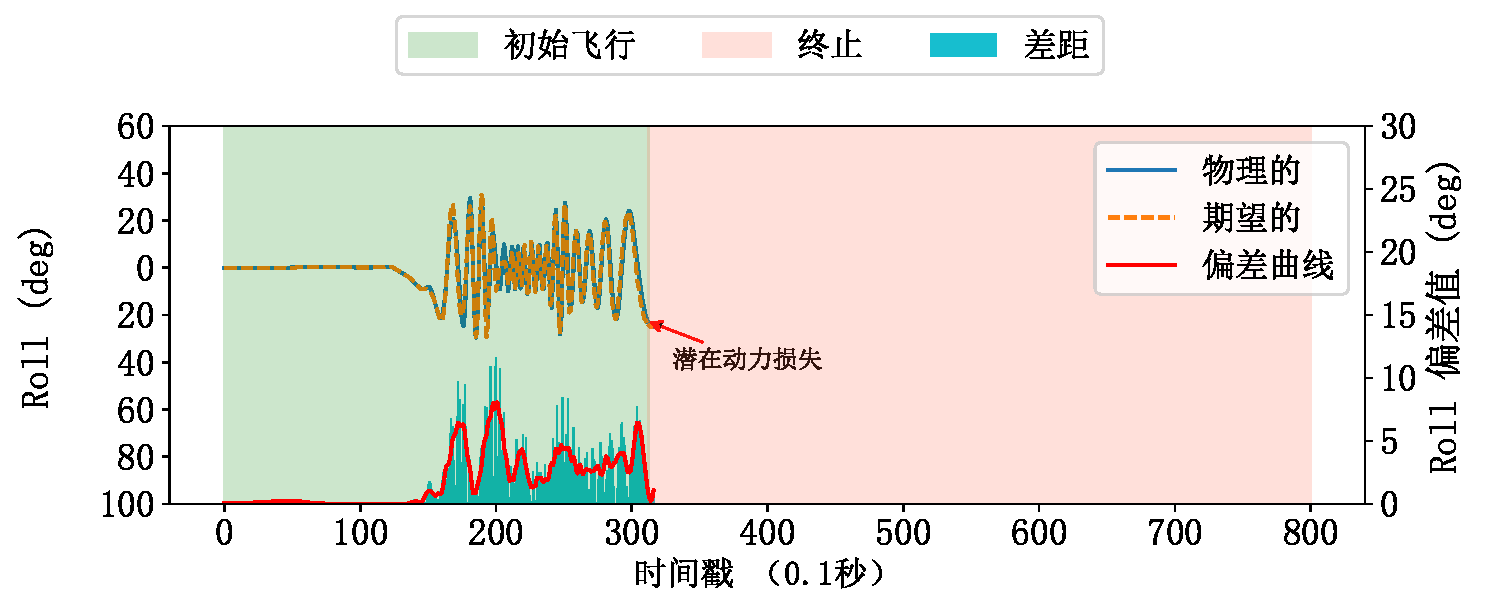
\includegraphics[width=\linewidth]{fig/fix/fix/raw_thrust_roll.pdf}\quad
    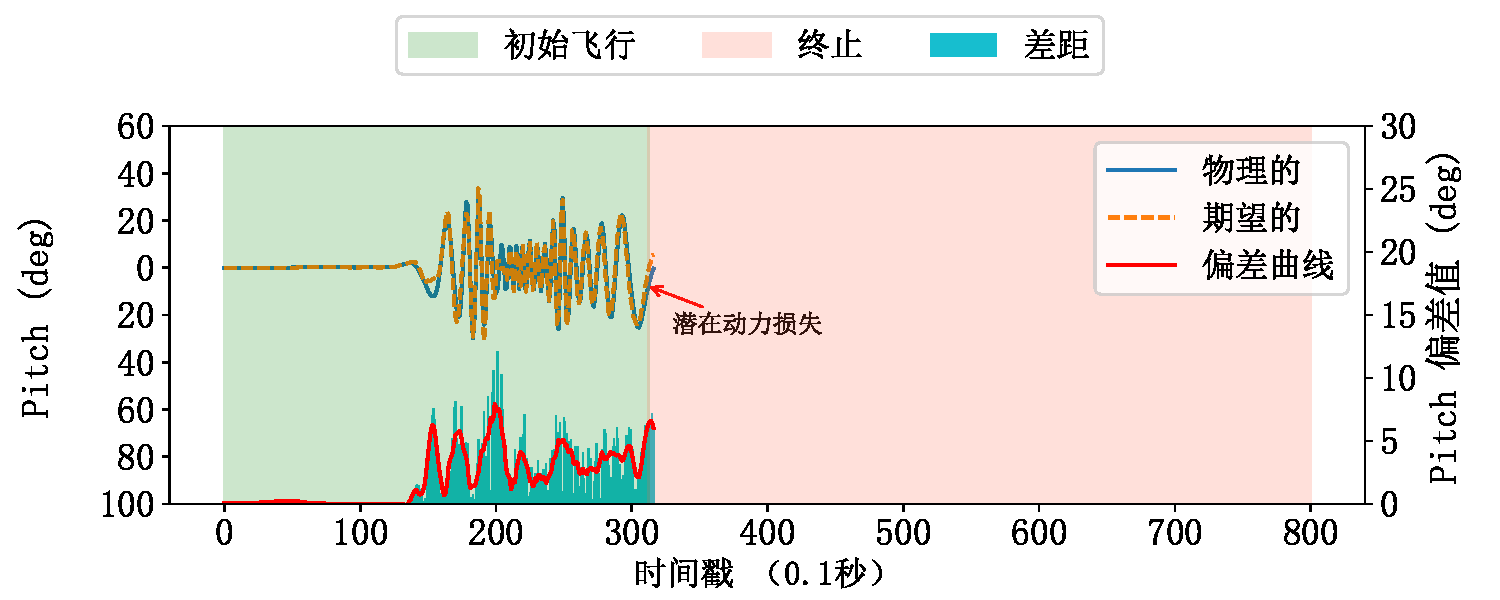
\includegraphics[width=\linewidth]{fig/fix/fix/raw_thrust_pitch.pdf}\quad
    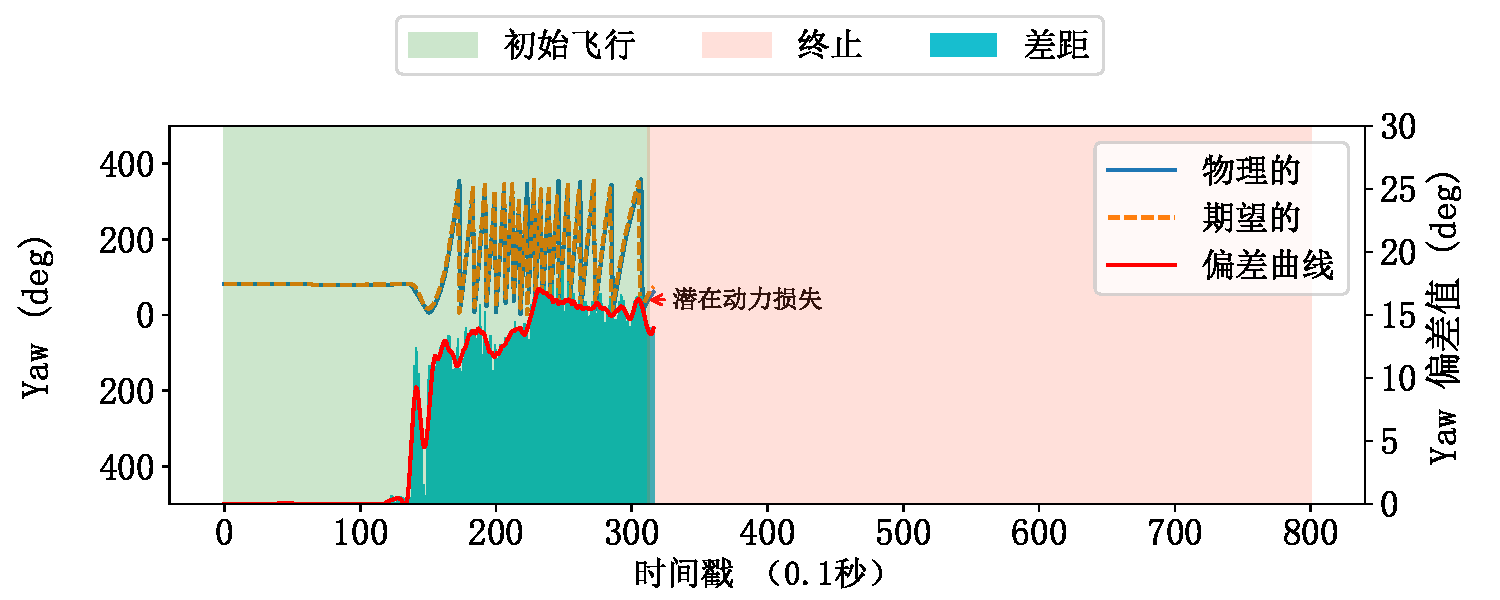
\includegraphics[width=\linewidth]{fig/fix/fix/raw_thrust_yaw.pdf}
    \caption{未装备\nyctea 无人机的状态}
    \label{subfig:fix_thurst_raw}
\end{minipage}
\begin{minipage}{0.49\linewidth}
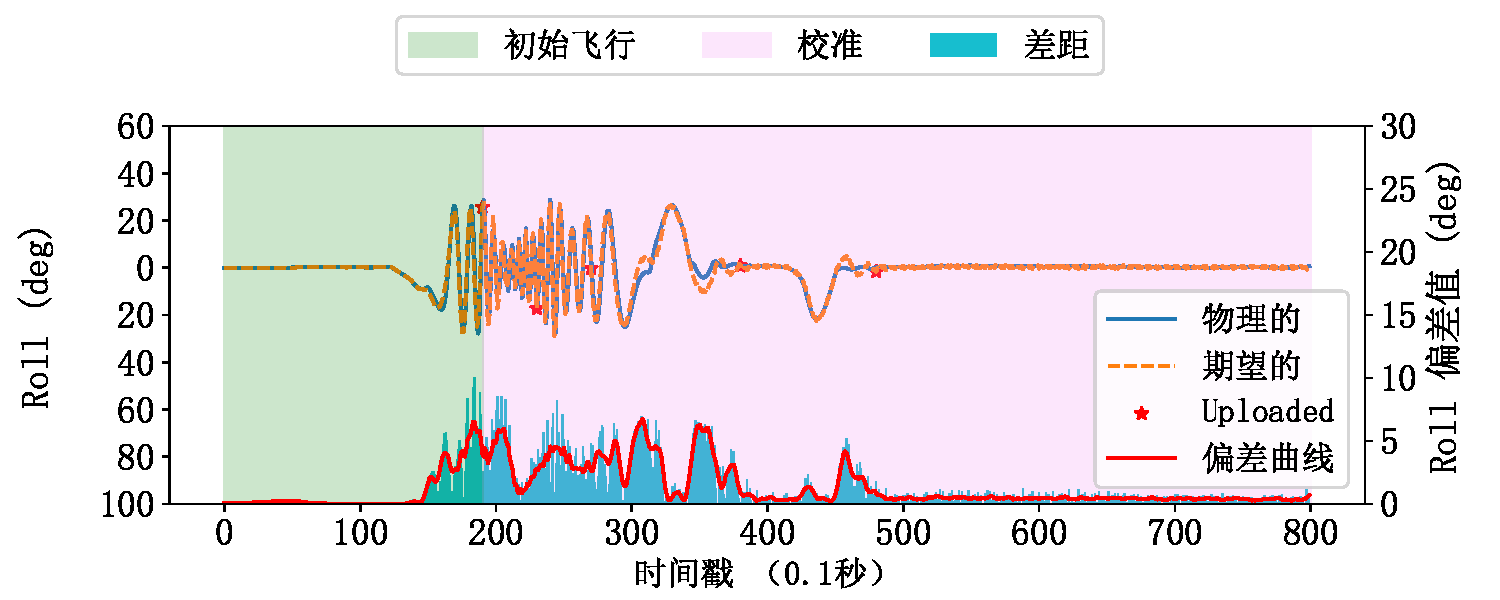
\includegraphics[width=\linewidth]{fig/fix/fix/fix_thrust_roll.pdf}\quad
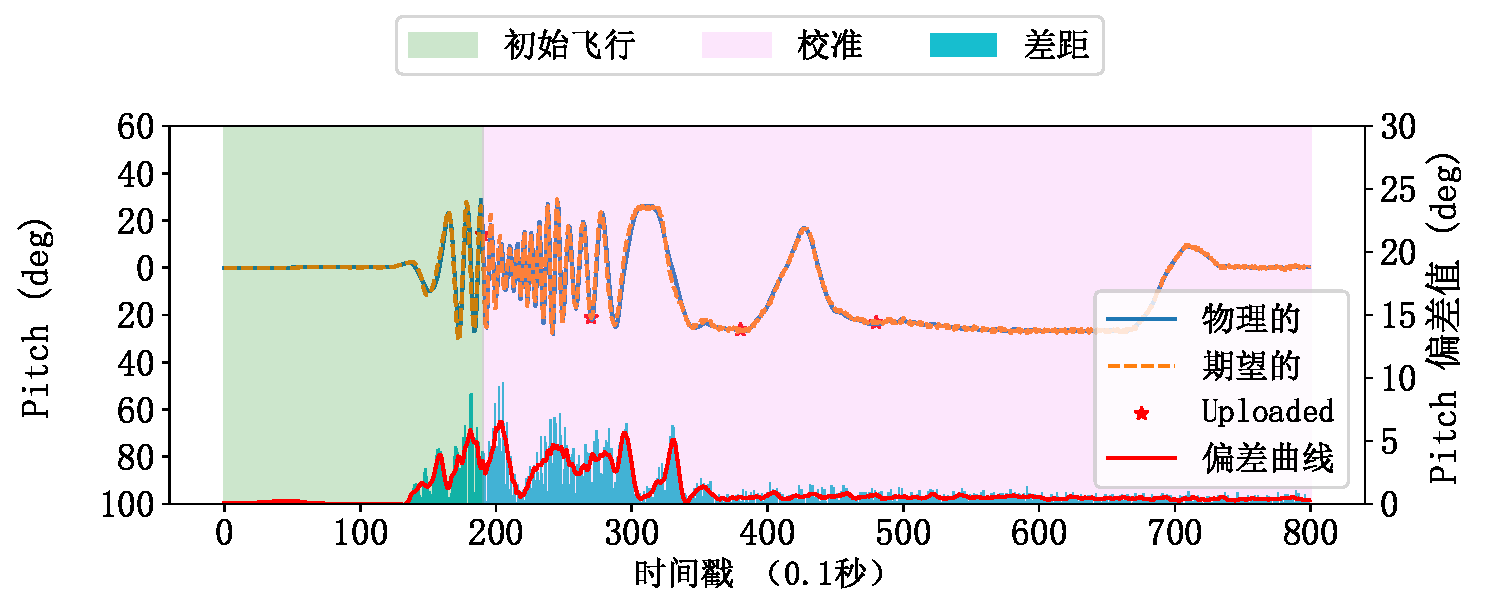
\includegraphics[width=\linewidth]{fig/fix/fix/fix_thrust_pitch.pdf}\quad
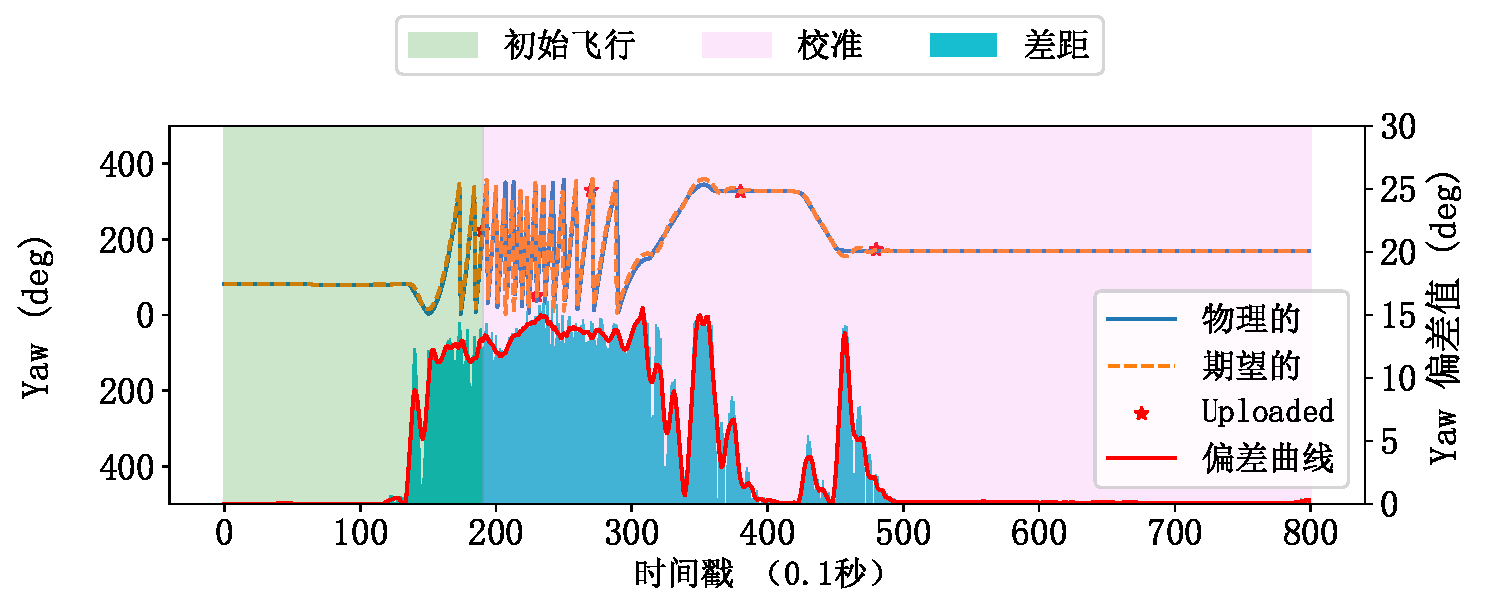
\includegraphics[width=\linewidth]{fig/fix/fix/fix_thrust_yaw.pdf}
\caption{未装备\nyctea 无人机的状态}
\label{subfig:fix_repair}
\end{minipage}


\end{figure*}

在第二个现实样例中,实验使用真实的无人机(\tool{CUAV ZD550})来测试\nyctea 的真实表现。 
整个不正确配置造成的相应的状态变化可以在图~\ref{fig:fix_deviation_change_real}中观察到。
在飞行过程中,物理状态在接受了配置后逐渐变得不稳定,并在到达任务航路点后开始振动。
\nyctea 识别出不稳定的物理状态并启动了第一次矫正(第一个 \emph{uploaded} 标记)。
虽然矫正减少了偏差,但并没有完全缓解问题。
\nyctea 生成了另一次矫正(第二个 \emph{uploaded} 标记),使无人机能够重新获得稳定飞行并成功完成任务。
总的来说,\nyctea 系统可以有效地识别和矫正现实飞行场景中的不稳定问题。


\begin{figure}[htb]
\centering{
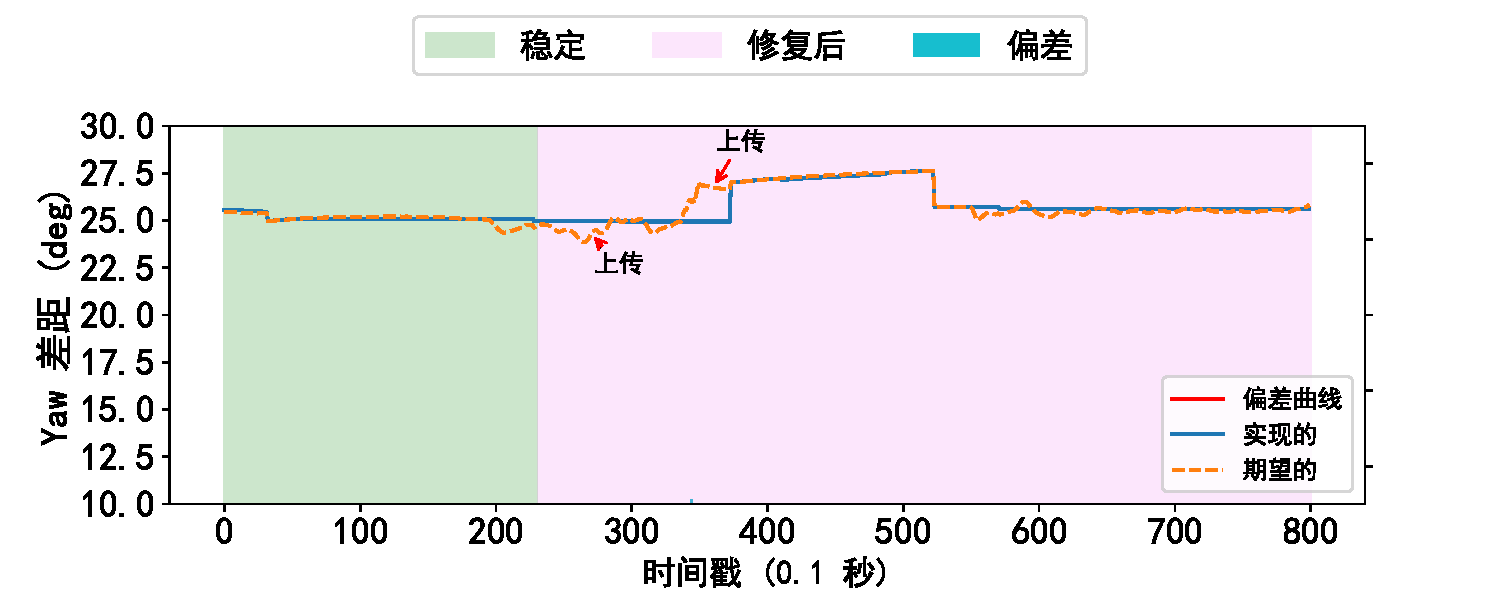
\includegraphics[width=0.98\linewidth]{fig/fix/fix/real_repair.pdf}}
\caption{真实无人机的 \nyctea 校正示例}
\label{fig:fix_deviation_change_real}
\end{figure}


\section{本章小结}
当无人机受到配置攻击或者传感器攻击时,可能会出现坠毁或者其他严重的事故。
本章节提出了一种在线修复系统--\nyctea ,它能实时检测并矫正由攻击或用户错误引起的不稳定物理状态,以防止无人机飞行过程中出现最糟糕的情况。
该系统通过计算已实现状态与期望状态之间的段偏差值来有效识别不稳定状态,并利用强化学习为无人机生成适当的配置。
实验测试了证明了\nyctea 的效率和修复成功率,结果表明其修复性能良好。